\documentclass[9pt, a4paper]{article}

\usepackage{ctex}
\usepackage{float}
\usepackage[utf8]{inputenc}
\usepackage{geometry}
\usepackage{graphicx}
\usepackage{subcaption}
\usepackage{multirow}
\geometry{margin=2.5cm}

\usepackage{listings}
\usepackage[dvipsnames]{xcolor}
% 在导言区进行样式设置
\lstset{
  language=c, % 设置语言
  basicstyle=\ttfamily\small, % 设置字体族和大小
  breaklines=true, % 自动换行
  keywordstyle=\bfseries\color{Purple}, % C语言关键字:紫色粗体
  morekeywords={uint32_t,uint8_t,float,char,static,const}, % C语言扩展关键字
  emph=[1]{delay_init,key_init,lcd_init,infrared_init,rgb_init,buzzer_init,led_init,usart_init,htu21d_init,fan_pwm_init}, % 初始化函数
  emphstyle=[1]\bfseries\color{Red}, % 初始化函数:红色粗体
  emph=[2]{htu21d_t,htu21d_h,get_infrared_status,fan_pwm_control,rgb_ctrl,led_control,buzzer_tweet}, % 硬件控制函数
  emphstyle=[2]\bfseries\color{Orange}, % 硬件控制函数:橙色粗体
  emph=[3]{update_display,get_centered_x,check_uart_command,send_system_status,auto_control,check_human_presence}, % 逻辑函数
  emphstyle=[3]\bfseries\color{Blue}, % 逻辑函数:蓝色粗体
  emph=[4]{sprintf,printf,strncmp,strlen,delay_ms,delay_count}, % 标准库函数
  emphstyle=[4]\color{Magenta}, % 标准库函数:洋红色
  commentstyle=\itshape\color{ForestGreen}, % 注释:森林绿斜体
  stringstyle=\color{Maroon}, % 字符串:栗色
  directivestyle=\color{Brown}, % 预处理器指令:棕色
  identifierstyle=\color{Black}, % 标识符:黑色
  numberstyle=\tiny\color{Gray}, % 数字:灰色小字
  columns=flexible,
  numbers=left, % 显示行号在左边
  numbersep=1.5em, % 设置行号的具体位置
  numberstyle=\footnotesize\color{Gray}, % 行号样式
  frame=single, % 边框
  framesep=1em, % 设置代码与边框的距离
  rulecolor=\color{lightgray}, % 边框颜色
  backgroundcolor=\color{Gray!5}, % 背景色:淡灰色
  tabsize=4, % Tab键宽度
  showstringspaces=false % 不显示字符串中的空格标记
}

\linespread{1}

\begin{document}

{
  \centering
  \fontsize{20pt}{24pt}\selectfont 温州理工学院

  \fontsize{15pt}{30pt}\selectfont \underline{嵌入式开发综合实践}实验报告

  \begin{table}[H]
    \centering
    \fontsize{12pt}{14pt}\selectfont
    \begin{tabular}{|c|c|c|c|c|c|}
      \hline
      \textbf{实验名称:} & \multicolumn{5}{c|}{\textbf{嵌入式开发综合实践设计说明书}} \\
      \hline
      \textbf{班~~级:} & \textbf{23计科三班} & \textbf{姓~~名:} & \textbf{程奕扬} & \textbf{学~~号:} & \textbf{23219111301} \\
      \hline
      \textbf{实验地点:} & \textbf{实3-1-205} & \textbf{日~~期:} & \multicolumn{3}{c|}{\textbf{2025年6月10日星期二}} \\
      \hline
    \end{tabular}
  \end{table}
}

\raggedright

\section{考核目标}

\begin{itemize}
    \vspace{-6pt}
  \item[1.] 进一步熟悉和掌握STM32的结构及工作原理。
    \vspace{-6pt}
  \item[2.] 掌握嵌入式主要接口和传感器驱动的开发技术。
    \vspace{-6pt}
  \item[3.] 通过程序设计,掌握以STM32F4系列芯片为核心的嵌入式软件的开发流程。
    \vspace{-6pt}
  \item[4.] 通过实际课程设计和调试,逐步掌握模块化程序设计方法和调试技术。
\end{itemize}

\section{实验环境}

\begin{itemize}
    \vspace{-6pt}
  \item 硬件环境: PC机Pentium处理器双核2GHz以上,内存4GB以上
    \vspace{-6pt}
  \item 操作系统: Windows10 64位操作系统
    \vspace{-6pt}
  \item 开发软件: IAR for ARM 集成开发环境
    \vspace{-6pt}
  \item 实验器材: 嵌入式原型机板卡ZI-ARMEmbed
    \vspace{-6pt}
  \item 实验配件: ARM仿真器、MiniUSB线、DC 12V电源
\end{itemize}

\section{方案论证与设计}

\subsection{需求分析与论证}

\subsubsection{项目背景与目标}

\qquad 随着物联网技术的发展和人们对智能化生活需求的不断提升,传统的风扇控制方式已无法满足现代用户对舒适度和节能的双重要求。本项目旨在设计并实现一款基于STM32F4xx微控制器的智能风扇控制系统,通过集成多种传感器和智能控制算法,实现风扇的自动化和智能化管理。

\subsubsection{功能需求分析}

\textbf{1. 核心控制功能需求}
\begin{itemize}
    \vspace{-6pt}
  \item \textbf{温度自适应控制}:系统需能够根据环境温度自动调节风扇转速,实现智能化温控
    \vspace{-6pt}
  \item \textbf{多档位风速控制}:支持0-3档风速调节,对应PWM占空比为0\%、33\%、66\%、100\%
    \vspace{-6pt}
  \item \textbf{双模式运行}:支持自动模式和手动模式切换,满足不同使用场景需求
\end{itemize}

\textbf{2. 人机交互功能需求}

\begin{itemize}
    \vspace{-6pt}
  \item \textbf{LCD显示界面}:实时显示温湿度、风扇转速、工作模式等关键信息
    \vspace{-6pt}
  \item \textbf{按键操控功能}:提供K1-K4四个按键,分别实现档位调节、模式切换、系统开关等功能
    \vspace{-6pt}
  \item \textbf{状态指示功能}:通过RGB LED和蜂鸣器提供直观的状态反馈
\end{itemize}

\textbf{3. 智能感知功能需求}

\begin{itemize}
    \vspace{-6pt}
  \item \textbf{环境监测}:集成HTU21D传感器,实现温湿度的精确测量
    \vspace{-6pt}
  \item \textbf{通信接口}:支持UART串口通信,可接收外部控制指令
\end{itemize}

\subsection{方案设计}

\subsubsection{硬件方案}

\qquad 本智能风扇控制系统采用模块化硬件设计,以STM32F4xx系列微控制器为核心,集成多种传感器和执行器件,构建完整的智能控制平台。

\textbf{1. 核心控制模块}
\begin{itemize}
    \vspace{-6pt}
  \item \textbf{主控芯片}:STM32F4xx系列微控制器,工作频率168MHz
    \vspace{-6pt}
  \item \textbf{系统时钟}:采用外部晶振,提供稳定的系统时钟源
    \vspace{-6pt}
  \item \textbf{电源管理}:DC 12V外部电源供电,内部稳压电路提供3.3V工作电压
\end{itemize}

\textbf{2. 传感器模块}
\begin{itemize}
    \vspace{-6pt}
  \item \textbf{温湿度传感器}:HTU21D数字传感器,I2C通信接口
    \begin{itemize}
        \vspace{-3pt}
      \item 温度测量范围:-40°C至+125°C,精度±0.3°C
        \vspace{-3pt}
      \item 湿度测量范围:0-100\%RH,精度±2\%RH
    \end{itemize}
    \vspace{-6pt}
\end{itemize}

\textbf{3. 人机交互模块}
\begin{itemize}
    \vspace{-6pt}
  \item \textbf{LCD显示屏}:320×240像素彩色LCD显示器
    \begin{itemize}
        \vspace{-3pt}
      \item 实时显示温湿度、风扇转速、工作模式
        \vspace{-3pt}
      \item 支持中文字符显示,具备文字居中对齐功能
    \end{itemize}
    \vspace{-6pt}
  \item \textbf{按键输入}:4个独立按键,支持中断触发
    \begin{itemize}
        \vspace{-3pt}
      \item K1:手动模式下风扇档位增加
        \vspace{-3pt}
      \item K2:手动模式下风扇档位减少
        \vspace{-3pt}
      \item K3:自动/手动模式切换
        \vspace{-3pt}
      \item K4:系统电源开关
    \end{itemize}
    \vspace{-6pt}
  \item \textbf{状态指示}:RGB LED灯和蜂鸣器
    \begin{itemize}
        \vspace{-3pt}
      \item RGB LED:不同颜色指示风扇运行状态
        \vspace{-3pt}
      \item 蜂鸣器:按键确认和高温警报提示
    \end{itemize}
\end{itemize}

\textbf{4. 执行器模块}
\begin{itemize}
    \vspace{-6pt}
  \item \textbf{风扇控制}:PWM调速控制,支持0-100\%无级调速
    \begin{itemize}
        \vspace{-3pt}
      \item PWM频率:50kHz,确保静音运行
        \vspace{-3pt}
      \item 档位设置:0档(0\%)、1档(33\%)、2档(66\%)、3档(100\%)
    \end{itemize}
    \vspace{-6pt}
  \item \textbf{指示灯控制}:D1/D2 LED指示当前工作模式
\end{itemize}

\textbf{5. 通信接口模块}
\begin{itemize}
    \vspace{-6pt}
  \item \textbf{UART串口}:波特率115200bps,支持远程控制命令
    \begin{itemize}
        \vspace{-3pt}
      \item 接收命令:"Auto"切换自动模式,"Manual"切换手动模式
        \vspace{-3pt}
      \item 发送状态:定时输出系统状态和传感器数据
    \end{itemize}
\end{itemize}

\subsubsection{软件方案}

\qquad 软件系统采用模块化设计思想,基于前后台程序架构,结合中断服务程序实现实时响应。系统软件分为初始化模块、控制逻辑模块、通信模块和显示模块等。

\textbf{1. 系统架构设计}
\begin{itemize}
    \vspace{-6pt}
  \item \textbf{主程序架构}:采用无限循环的前台程序结构
    \begin{itemize}
        \vspace{-3pt}
      \item 主循环周期:1ms,确保系统实时响应
        \vspace{-3pt}
      \item 任务调度:基于时间片轮询的任务调度机制
    \end{itemize}
    \vspace{-6pt}
  \item \textbf{中断处理}:按键中断优先级最高,确保用户操作及时响应
    \begin{itemize}
        \vspace{-3pt}
      \item 按键防抖:50ms软件防抖处理
        \vspace{-3pt}
      \item 中断标志:通过全局变量进行中断事件传递
    \end{itemize}
\end{itemize}

\textbf{2. 状态机设计}
\begin{itemize}
    \vspace{-6pt}
  \item \textbf{系统状态}:系统开/关两种基本状态
    \begin{itemize}
        \vspace{-3pt}
      \item 开机状态:正常执行所有功能模块
        \vspace{-3pt}
      \item 关机状态:停止风扇运行,保持状态监测
    \end{itemize}
    \vspace{-6pt}
  \item \textbf{工作模式}:自动模式和手动模式
    \begin{itemize}
        \vspace{-3pt}
      \item 自动模式:根据温度阈值自动调节风扇档位
        \vspace{-3pt}
      \item 手动模式:用户通过按键手动设置风扇档位
    \end{itemize}
    \vspace{-6pt}
\end{itemize}

\textbf{3. 控制算法}
\begin{itemize}
    \vspace{-6pt}
  \item \textbf{温度控制算法}:基于温度阈值的分档控制
    \begin{itemize}
        \vspace{-3pt}
      \item 高温区(≥30°C):3档风速,蜂鸣器报警
        \vspace{-3pt}
      \item 中温区(25-29°C):2档风速
        \vspace{-3pt}
      \item 低温区(20-24°C):1档风速
        \vspace{-3pt}
      \item 舒适区(<20°C):关闭风扇
    \end{itemize}
    \vspace{-6pt}

\end{itemize}

\textbf{4. 数据处理}
\begin{itemize}
    \vspace{-6pt}
  \item \textbf{传感器数据采集}:HTU21D传感器I2C通信
    \begin{itemize}
        \vspace{-3pt}
      \item 采样频率:根据需要实时读取
        \vspace{-3pt}
      \item 数据格式:浮点数格式存储温湿度值
    \end{itemize}
    \vspace{-6pt}
  \item \textbf{显示数据处理}:LCD显示的字符串格式化
    \begin{itemize}
        \vspace{-3pt}
      \item 文字居中算法:自动计算中英文混合字符串的居中位置
        \vspace{-3pt}
      \item 数据格式化:温度显示2位小数,湿度显示1位小数
    \end{itemize}
\end{itemize}

\subsubsection{函数定义总览}

\qquad 系统软件共定义了多个功能函数,按照模块进行分类管理,实现代码的模块化和可维护性。

\textbf{1. 系统初始化函数}
\begin{itemize}
    \vspace{-6pt}
  \item \texttt{delay\_init(168)}:延时系统初始化,设置系统时钟
    \vspace{-6pt}
  \item \texttt{key\_init()}:按键GPIO初始化
    \vspace{-6pt}
  \item \texttt{key\_interrupt\_init()}:按键中断初始化配置
    \vspace{-6pt}
  \item \texttt{lcd\_init(FAN1)}:LCD显示器初始化
    \vspace{-6pt}
  \item \texttt{infrared\_init()}:红外传感器初始化
    \vspace{-6pt}
  \item \texttt{rgb\_init()}:RGB LED初始化
    \vspace{-6pt}
  \item \texttt{buzzer\_init()}:蜂鸣器初始化
    \vspace{-6pt}
  \item \texttt{led\_init()}:指示LED初始化
    \vspace{-6pt}
  \item \texttt{usart\_init(115200)}:串口通信初始化
    \vspace{-6pt}
  \item \texttt{htu21d\_init()}:温湿度传感器初始化
    \vspace{-6pt}
  \item \texttt{fan\_pwm\_init(50000-1, 336-1)}:风扇PWM初始化
\end{itemize}

\textbf{2. 传感器数据采集函数}
\begin{itemize}
    \vspace{-6pt}
  \item \texttt{float htu21d\_t()}:读取温度传感器数据,返回摄氏度值
    \vspace{-6pt}
  \item \texttt{float htu21d\_h()}:读取湿度传感器数据,返回百分比值
\end{itemize}

\textbf{3. 显示控制函数}
\begin{itemize}
    \vspace{-6pt}
  \item \texttt{int get\_centered\_x(const char *text)}:计算文字居中显示的X坐标
    \begin{itemize}
        \vspace{-3pt}
      \item 功能:智能识别中英文字符,自动计算居中位置
        \vspace{-3pt}
      \item 算法:中文字符16像素宽,英文字符8像素宽
    \end{itemize}
    \vspace{-6pt}
  \item \texttt{void update\_display(float temp, float humi)}:更新LCD显示内容
    \begin{itemize}
        \vspace{-3pt}
      \item 显示内容:风扇转速、工作模式、温湿度数据
        \vspace{-3pt}
      \item 系统状态:区分开机/关机状态的不同显示内容
    \end{itemize}
\end{itemize}

\textbf{4. 通信处理函数}
\begin{itemize}
    \vspace{-6pt}
  \item \texttt{void check\_uart\_command()}:检查并处理串口接收命令
    \begin{itemize}
        \vspace{-3pt}
      \item 支持命令:"Auto"切换自动模式,"Manual"切换手动模式
        \vspace{-3pt}
      \item 响应机制:命令执行后发送确认信息并更新显示
    \end{itemize}
    \vspace{-6pt}
  \item \texttt{void send\_system\_status(float temp, float humi)}:发送系统状态信息
    \begin{itemize}
        \vspace{-3pt}
      \item 状态内容:风扇状态、工作模式、转速、温湿度
        \vspace{-3pt}
      \item 发送周期:每3ms发送一次状态更新
    \end{itemize}
    \vspace{-6pt}
  \item \texttt{clean\_usart()}:清空串口接收缓冲区
\end{itemize}

\textbf{5. 控制逻辑函数}
\begin{itemize}
    \vspace{-6pt}
  \item \texttt{void auto\_control(float temp, float humi)}:自动模式控制逻辑
    \begin{itemize}
        \vspace{-3pt}
      \item 温度判断:根据预设阈值自动调节风扇档位
        \vspace{-3pt}
      \item 状态指示:控制RGB LED和蜂鸣器状态
        \vspace{-3pt}
      \item 安全保护:高温时蜂鸣器报警(最多3次)
    \end{itemize}
    \vspace{-6pt}
  \item \texttt{fan\_pwm\_control(fan\_pwm[count])}:风扇PWM控制输出
    \vspace{-6pt}
  \item \texttt{rgb\_ctrl()}:RGB指示灯控制
    \vspace{-6pt}
  \item \texttt{led\_control()}:模式指示LED控制
    \vspace{-6pt}
  \item \texttt{buzzer\_tweet()}:蜂鸣器控制
\end{itemize}

\textbf{6. 辅助工具函数}
\begin{itemize}
    \vspace{-6pt}
  \item \texttt{void delay\_count(uint32\_t times)}:自定义计数延时函数
    \begin{itemize}
        \vspace{-3pt}
      \item 用途:按键防抖延时,精确时间控制
        \vspace{-3pt}
      \item 实现:基于循环计数的软件延时
    \end{itemize}
    \vspace{-6pt}
  \item \texttt{delay\_ms()}:毫秒级延时函数
    \vspace{-6pt}
  \item \texttt{sprintf()}:字符串格式化函数
    \vspace{-6pt}
  \item \texttt{printf()}:串口输出函数
    \vspace{-6pt}
  \item \texttt{strncmp()}:字符串比较函数
\end{itemize}

\qquad 整个软件系统通过合理的函数模块划分,实现了硬件抽象、逻辑控制和人机交互的有效分离,提高了代码的可读性、可维护性和可扩展性。各模块之间通过标准接口进行数据交换,确保系统的稳定性和可靠性。

\section{程序设计}

\subsection{系统初始化模块}

\begin{lstlisting}
    /****************************************
    *          系统初始化模块开始           *
    ****************************************/

   char buf[30] = {0};
   float current_temp;
   float current_humi;

   // 硬件模块初始化
   delay_init(168);
   key_init();
   key_interrupt_init();
   lcd_init(FAN1);
   infrared_init();
   rgb_init();
   buzzer_init();
   led_init();
   usart_init(115200);
   htu21d_init();
   fan_pwm_init(50000 - 1, 336 - 1);

   /****************************************
    *        LCD初始化显示模块开始         *
    ****************************************/

   // LCD界面初始化显示 - 显示基本标签和初始值
   sprintf(buf, "Fan PWM:%3d%%", fan_pwm[count]);
   LCDDrawFont16_Next(get_centered_x(buf), 20 + 10 * 7, 4, 320, buf, 0x0000,
                      0xffff); // 显示初始PWM值
   LCDDrawFont16_Next(get_centered_x("Mode:"), 30 + 10 * 8, 4, 320,
                      "Mode:", 0x0000, 0xffff); // 显示模式标签
   LCDDrawFont16_Next(get_centered_x("Temp:"), 30 + 10 * 10, 4, 320,
                      "Temp:", 0x0000, 0xffff); // 显示温度标签
   LCDDrawFont16_Next(get_centered_x("Humi:"), 30 + 10 * 12, 4, 320,
                      "Humi:", 0x0000, 0xffff); // 显示湿度标签
\end{lstlisting}

\subsection{温、湿度检测模块}

\begin{lstlisting}
    /*********************************************************
    * 功能:读取温度
    * 参数:无
    * 返回:-1/float t -- 处理后的温度值
    **********************************************************/
   float htu21d_t(void) {
     char cmd = 0xf3;
     char dat[4];
     i2c_write(HTU21D_ADDR, &cmd, 1);
     delay_ms(50);
     if (i2c_read(HTU21D_ADDR, dat, 2) == 2) {
       if ((dat[1] & 0x02) == 0) {
         float t =
             -46.85f + 175.72f * ((dat[0] << 8 | dat[1]) & 0xfffc) / (1 << 16);
         return t;
       }
     }
     return -1;
   }

   /************************************************************
    * 名称:htu21d_h()
    * 功能:读取湿度
    * 参数:无
    * 返回:-1/float h -- 处理后的湿度值
    ************************************************************/
   float htu21d_h(void) {
     char cmd = 0xf5;
     char dat[4];

     i2c_write(HTU21D_ADDR, &cmd, 1);
     delay_ms(50);
     if (i2c_read(HTU21D_ADDR, dat, 2) == 2) {
       if ((dat[1] & 0x02) == 0x02) {
         float h = -6 + 125 * ((dat[0] << 8 | dat[1]) & 0xfffc) / (1 << 16);
         return h;
       }
     }
     return -1;
   }
\end{lstlisting}

\subsection{UART通信模块}

\begin{lstlisting}
    /****************************************
    *          UART通信模块开始            *
    ****************************************/

   void check_uart_command(void) {
     // 检查串口接收缓冲区是否有足够的数据
     if (Usart_len >= 4) {
       // 检查是否接收到"Auto"命令
       if (strncmp((char *)USART_RX_BUF, "Auto", 4) == 0) {
         mode = AUTO_MODE;
         led_control(D2);
         printf("Mode switched to Auto\r\n");
         update_display(htu21d_t(), htu21d_h());
       }
       // 检查是否接收到"Manual"命令
       else if (strncmp((char *)USART_RX_BUF, "Manual", 6) == 0) {
         mode = MANUAL_MODE;
         led_control(D1);
         printf("Mode switched to Manual\r\n");
         update_display(htu21d_t(), htu21d_h());
       }
       // 清空串口接收缓冲区
       clean_usart();
     }
   }
\end{lstlisting}

\subsection{风扇模块}

\begin{lstlisting}
    /************************************************************
    * 功能:风扇传感器初始化
    * 参数:无
    * 返回:无
    *************************************************************/
   void fan_init(void) {
     GPIO_InitTypeDef GPIO_InitStructure; // 定义一个GPIO_InitTypeDef类型的结构体
     RCC_AHB1PeriphClockCmd(RCC_AHB1Periph_GPIOE,
                            ENABLE); // 开启风扇传感器相关的GPIO外设时钟

     GPIO_InitStructure.GPIO_Pin = GPIO_Pin_5;        // 选择要控制的GPIO引脚
     GPIO_InitStructure.GPIO_OType = GPIO_OType_PP;   // 设置引脚的输出类型为推挽
     GPIO_InitStructure.GPIO_Mode = GPIO_Mode_OUT;    // 设置引脚模式为输出模式
     GPIO_InitStructure.GPIO_PuPd = GPIO_PuPd_DOWN;   // 设置引脚为下拉模式
     GPIO_InitStructure.GPIO_Speed = GPIO_Speed_2MHz; // 设置引脚速率为2MHz

     GPIO_Init(GPIOE, &GPIO_InitStructure); // 初始化GPIO配置
     GPIO_ResetBits(GPIOE, GPIO_Pin_5);
   }

   /**************************************************************
    * 名称:void fan_control(unsigned char cmd)
    * 功能:风扇控制驱动
    * 参数:控制命令
    * 返回:无
    **************************************************************/
   void fan_control(unsigned char cmd) {
     if (cmd & 0x01)
       GPIO_SetBits(GPIOE, GPIO_Pin_5);
     else
       GPIO_ResetBits(GPIOE, GPIO_Pin_5);
   }

   static u32 cycle; // 这个值不要小于100,否则占空比不准确
   /***************************************************************
    * 名称:fan_pwm_init()
    * 功能:风扇传感器PWM初始化  PE5 连接 TIM9——CH1  16位定时器
    * 参数:arr:自动重装值  psc:时钟预分频数
    * 返回:无
    ***************************************************************/
   void fan_pwm_init(u32 arr, u32 psc) {
     cycle = arr + 1; // 用来计算占空比。需要加1
     // 此部分需手动修改IO口设置
     GPIO_InitTypeDef GPIO_InitStructure = {0};
     TIM_TimeBaseInitTypeDef TIM_TimeBaseStructure = {0};
     TIM_OCInitTypeDef TIM_OCInitStructure = {0};

     RCC_APB2PeriphClockCmd(RCC_APB2Periph_TIM9, ENABLE);  // TIM9时钟使能
     RCC_AHB1PeriphClockCmd(RCC_AHB1Periph_GPIOE, ENABLE); // 使能PORTF时钟

     GPIO_PinAFConfig(GPIOE, GPIO_PinSource5, GPIO_AF_TIM9); // GPIOE5
                                                             // 复用为定时器9

     GPIO_InitStructure.GPIO_Pin = GPIO_Pin_5;          // GPIOE5
     GPIO_InitStructure.GPIO_Mode = GPIO_Mode_AF;       // 复用功能
     GPIO_InitStructure.GPIO_Speed = GPIO_Speed_100MHz; // 速度100MHz
     GPIO_InitStructure.GPIO_OType = GPIO_OType_PP;     // 推挽复用输出
     GPIO_InitStructure.GPIO_PuPd = GPIO_PuPd_UP;       // 上拉
     GPIO_Init(GPIOE, &GPIO_InitStructure);             // 初始化PE5

     TIM_TimeBaseStructure.TIM_Prescaler =
         psc; // 定时器分频,定时器9挂载到APB2,为168MHZ,如果这里分频到1MHZ,设置为167
     TIM_TimeBaseStructure.TIM_CounterMode = TIM_CounterMode_Up; // 向上计数模式
     TIM_TimeBaseStructure.TIM_Period = arr;                     // 自动重装载值
     TIM_TimeBaseStructure.TIM_ClockDivision = TIM_CKD_DIV1;
     TIM_TimeBaseInit(TIM9, &TIM_TimeBaseStructure); // 初始化定时器9

     // 初始化TIM9 Channel1 PWM模式
     TIM_OCInitStructure.TIM_OCMode =
         TIM_OCMode_PWM1; // 选择定时器模式:TIM脉冲宽度调制模式
     TIM_OCInitStructure.TIM_OutputState = TIM_OutputState_Enable; // 比较输出使能
     TIM_OCInitStructure.TIM_OCPolarity = TIM_OCPolarity_High;     // 输出极性
     TIM_OC1Init(TIM9, &TIM_OCInitStructure);                      // 初始化通道1

     TIM_OC1PreloadConfig(TIM9,
                          TIM_OCPreload_Enable); // 使能TIM在CCR1上的预装载寄存器

     TIM_ARRPreloadConfig(TIM9, ENABLE); // ARPE使能
     TIM_Cmd(TIM9, ENABLE);              // 使能TIM
   }

   /******************************************************************
    * 名称:fan_pwm_control
    * 功能:风扇PWM驱动控制
    * 参数:pwm 占空比 0-100
    * 返回:无
    ******************************************************************/
   void fan_pwm_control(uint32_t pwm) {
     uint32_t _pwm = cycle / 100 * pwm;
     TIM_SetCompare1(TIM9, _pwm); // 修改比较值,修改占空比
   }
\end{lstlisting}

\subsection{风扇自动控制模块}

\begin{lstlisting}[caption={自动调控逻辑}]
 /****************************************
 *         风扇自动控制模块开始          *
 ****************************************/

void auto_control(float temp, float humi) {
  char new_count;

  // 根据温度范围自动调节风扇档位
  if (temp >= TEMP_HIGH) { // 温度 >= 30°C,高速档
    new_count = 3;
    // 只在最高档时响3下蜂鸣器,和手动模式保持一致
    if (buzzer_count < 3) {
      buzzer_tweet();
      buzzer_count++;
    }
    rgb_ctrl(5);                 // 设置RGB指示灯为高温状态
  } else if (temp >= TEMP_MED) { // 温度 >= 25°C,中速档
    new_count = 2;
    buzzer_count = 0;            // 重置蜂鸣器计数
    rgb_ctrl(4);                 // 设置RGB指示灯为中温状态
  } else if (temp >= TEMP_LOW) { // 温度 >= 20°C,低速档
    new_count = 1;
    buzzer_count = 0; // 重置蜂鸣器计数
    rgb_ctrl(3);      // 设置RGB指示灯为低温状态
  } else {            // 温度 < 20°C,关闭风扇
    new_count = 0;
    buzzer_count = 0; // 重置蜂鸣器计数
    rgb_ctrl(2);      // 设置RGB指示灯为正常状态
  }

  // 如果档位发生变化,更新风扇控制和显示
  if (count != new_count) {
    count = new_count;
    update_display(temp, humi);
  }
}
\end{lstlisting}

\begin{lstlisting}[caption={模式匹配逻辑}]
    // 根据当前模式执行风扇控制策略
    if (mode == AUTO_MODE) {
      // 自动模式:根据温度自动调节风扇转速
      auto_control(current_temp, current_humi);
    } else {
      // 手动模式:根据用户设定的档位控制风扇和指示灯
      if (count == 3) { // 最高档位(100%)
        if (buzzer_count < 3) {
          buzzer_tweet(); // 最高档时蜂鸣器响3下提醒
          buzzer_count++;
        }
        rgb_ctrl(5);           // 高速档RGB指示灯
      } else if (count == 2) { // 中档位(66%)
        buzzer_count = 0;      // 重置蜂鸣器计数
        rgb_ctrl(4);           // 中速档RGB指示灯
      } else if (count == 1) { // 低档位(33%)
        buzzer_count = 0;      // 重置蜂鸣器计数
        rgb_ctrl(3);           // 低速档RGB指示灯
      } else if (count == 0) { // 关闭档位(0%)
        buzzer_count = 0;      // 重置蜂鸣器计数
        rgb_ctrl(2);           // 停止档RGB指示灯
      }
    }
\end{lstlisting}

\subsection{风扇手动控制模块}

\begin{lstlisting}
      if (mode == MANUAL_MODE && current_key == K1_PREESED) {
        // K1按键:手动模式下增加风扇档位
        count++;
        buzzer_tweet(); // 按键确认音
        if (count >= ARRAY(fan_pwm))
          count = ARRAY(fan_pwm) - 1; // 限制最大档位
        update_display(current_temp, current_humi);
      } else if (mode == MANUAL_MODE && current_key == K2_PREESED) {
        // K2按键:手动模式下减少风扇档位
        if (count > 0) {
          count--; // 减少档位
        }
        buzzer_tweet(); // 按键确认音
        update_display(current_temp, current_humi);
      }
\end{lstlisting}

\subsection{LCD显示模块}

\begin{lstlisting}[caption={主要信息显示}]
    /****************************************
    *          LCD显示模块开始             *
    ****************************************/

   void update_display(float temp, float humi) {
     char buf[100];

     // 系统关闭状态显示
     if (system_power == 0) {
       sprintf(buf, "---风扇已关闭-----");
       LCDDrawFont16_Next(get_centered_x(buf), 20 + 10 * 7, 4, 320, buf, 0x0000,
                          0xffff);
       LCDDrawFont16_Next(get_centered_x("---按下K4启动---"), 30 + 10 * 8, 4, 320,
                          "---按下K4启动---", 0x0000, 0xffff);
       // 清空其他显示行
       LCDDrawFont16_Next(get_centered_x(""), 30 + 10 * 10, 4, 320, "", 0x0000,
                          0xffff);
       LCDDrawFont16_Next(get_centered_x(""), 30 + 10 * 12, 4, 320, "", 0x0000,
                          0xffff);
       LCDDrawFont16_Next(get_centered_x(""), 30 + 10 * 14, 4, 320, "", 0x0000,
                          0xffff);
       return;
     }

     // 系统运行状态显示
     // 显示风扇转速和档位
     sprintf(buf, "风扇转速: %3d%%(%s)", fan_pwm[count], fan_pwm1[count]);
     LCDDrawFont16_Next(get_centered_x(buf), 20 + 10 * 7, 4, 320, buf, 0x0000,
                        0xffff);

     // 显示当前工作模式
     sprintf(buf, "风扇模式: %s",
             mode == AUTO_MODE ? "-自动-"
                               : (mode == MANUAL_MODE ? "-手动-" : "-自动-"));
     LCDDrawFont16_Next(get_centered_x(buf), 30 + 10 * 8, 4, 320, buf, 0x0000,
                        0xffff);

     // 显示当前温度
     sprintf(buf, "当前温度: %.2f °C", temp);
     LCDDrawFont16_Next(get_centered_x(buf), 30 + 10 * 10, 4, 320, buf, 0x0000,
                        0xffff);

     // 显示当前湿度
     sprintf(buf, "当前湿度: %.1f%%RH", humi);
     LCDDrawFont16_Next(get_centered_x(buf), 30 + 10 * 12, 4, 320, buf, 0x0000,
                        0xffff);
   }
\end{lstlisting}

\begin{lstlisting}[caption={实验标题显示}]
    /*****************************************************
    * 名称:lcd_init()
    * 功能:LCD初始化并打印实验基本信息
    * 参数:name -- 实验名称
    * 返回:无
    ******************************************************/
   void lcd_init(unsigned char name) {
     LCD_DriverInit();
     LCD_Clear(0xFFFF);
     LCD_FillColor(0, 0, 319, 30, 0x4596);
     LCDDrawFnt24(80, 5, "风扇智能调节系统", 0xFFD700, 0x4596);
     LCD_FillColor(0, 240 - 30, 319, 240, 0x4596);
     LCDDrawFnt24(96, 240 - 30 + 5, "嵌入式实践设计", 0xFFD700, 0x4596);
   }
\end{lstlisting}

\subsection{按键控制模块}

\begin{lstlisting}[caption={按键中断初始化}]
    void key_interrupt_init(void) {
        EXTI_InitTypeDef EXTI_InitStructure;
        NVIC_InitTypeDef NVIC_InitStructure;

        RCC_APB2PeriphClockCmd(RCC_APB2Periph_SYSCFG, ENABLE);

        SYSCFG_EXTILineConfig(EXTI_PortSourceGPIOB, EXTI_PinSource12);
        SYSCFG_EXTILineConfig(EXTI_PortSourceGPIOB, EXTI_PinSource13);
        SYSCFG_EXTILineConfig(EXTI_PortSourceGPIOB, EXTI_PinSource14);
        SYSCFG_EXTILineConfig(EXTI_PortSourceGPIOB, EXTI_PinSource15);

        EXTI_InitStructure.EXTI_Line =
            EXTI_Line12 | EXTI_Line13 | EXTI_Line14 | EXTI_Line15;
        EXTI_InitStructure.EXTI_Mode = EXTI_Mode_Interrupt;
        EXTI_InitStructure.EXTI_Trigger = EXTI_Trigger_Falling;
        EXTI_InitStructure.EXTI_LineCmd = ENABLE;
        EXTI_Init(&EXTI_InitStructure);

        NVIC_InitStructure.NVIC_IRQChannel = EXTI15_10_IRQn;
        NVIC_InitStructure.NVIC_IRQChannelPreemptionPriority = 0x02;
        NVIC_InitStructure.NVIC_IRQChannelSubPriority = 0x02;
        NVIC_InitStructure.NVIC_IRQChannelCmd = ENABLE;
        NVIC_Init(&NVIC_InitStructure);
      }

      void EXTI15_10_IRQHandler(void) {
        if (EXTI_GetITStatus(EXTI_Line12) != RESET) {
          EXTI_ClearITPendingBit(EXTI_Line12);
          key_value = K1_PREESED;
          key_interrupt_flag = 1;
        }
        if (EXTI_GetITStatus(EXTI_Line13) != RESET) {
          EXTI_ClearITPendingBit(EXTI_Line13);
          key_value = K2_PREESED;
          key_interrupt_flag = 1;
        }
        if (EXTI_GetITStatus(EXTI_Line14) != RESET) {
          EXTI_ClearITPendingBit(EXTI_Line14);
          key_value = K3_PREESED;
          key_interrupt_flag = 1;
        }
        if (EXTI_GetITStatus(EXTI_Line15) != RESET) {
          EXTI_ClearITPendingBit(EXTI_Line15);
          key_value = K4_PREESED;
          key_interrupt_flag = 1;
        }
      }
\end{lstlisting}

\begin{lstlisting}[caption={部分按键控制模块}]
    /****************************************
     *          按键控制模块开始            *
     ****************************************/

    // K4按键:系统电源开关控制
    if (key_interrupt_flag) {
      delay_count(50); // 按键防抖延时
      char current_key = key_value;
      key_interrupt_flag = 0;

      if (current_key == K4_PREESED) {
        system_power = !system_power; // 切换系统电源状态
        buzzer_tweet();               // 按键确认音
        if (system_power == 0) {
          count = 0;                       // 关闭时重置风扇档位
          fan_pwm_control(fan_pwm[count]); // 停止风扇
          rgb_ctrl(2);                     // 设置RGB为正常状态
        }
        update_display(htu21d_t(), htu21d_h());
        continue;
      }
    }
\end{lstlisting}

\subsection{蜂鸣器模块}

\begin{lstlisting}
    void buzzer_init(void)
    {
      GPIO_InitTypeDef GPIO_InitStructure;

      RCC_AHB1PeriphClockCmd(BUZZER_RCC, ENABLE);

      GPIO_InitStructure.GPIO_Mode = GPIO_Mode_OUT;
      GPIO_InitStructure.GPIO_OType = GPIO_OType_PP;
      GPIO_InitStructure.GPIO_PuPd = GPIO_PuPd_UP;
      GPIO_InitStructure.GPIO_Speed = GPIO_Speed_100MHz;

      GPIO_InitStructure.GPIO_Pin = BUZZER_PIN;
      GPIO_Init(BUZZER_PORT, &GPIO_InitStructure);

      BUZZER_CTRL(OFF);
    }

    void buzzer_tweet(void)
    {
      BUZZER_CTRL(ON);
      delay_ms(5);
      BUZZER_CTRL(OFF);
    }

    void buzzer_stop(void)
    {
      BUZZER_CTRL(OFF);  // 关闭蜂鸣器
    }
\end{lstlisting}

\newpage

\subsection{程序流程图}

\begin{figure}[htbp]
  \centering
  \includegraphics[width=\textwidth]{../figures/program-gra.png}
  \caption{程序流程图}
  \label{fig:1}
\end{figure}

\section{调试及性能分析}

\subsection{调试过程}

\qquad 智能风扇控制系统的调试工作按照模块化的思路进行,采用分模块测试、功能验证、集成调试的步骤,确保每个功能模块的正确性和系统整体的稳定性。

\subsubsection{系统初始化调试}

\qquad 系统初始化是整个项目的基础,包括STM32微控制器时钟配置、GPIO初始化、外设配置等关键环节。

\textbf{调试内容:}
\begin{itemize}
    \vspace{-6pt}
  \item 验证系统时钟频率设置(168MHz)是否正确
    \vspace{-6pt}
  \item 检查各外设模块初始化函数的执行状态
    \vspace{-6pt}
  \item 确认GPIO引脚配置与硬件连接的一致性
    \vspace{-6pt}
  \item 测试系统启动后的基本响应能力
\end{itemize}

\textbf{调试方法:}通过LED指示灯闪烁和串口输出信息验证系统成功启动,观察各初始化函数的返回值。

% 预留图片位置
\begin{figure}[H]
  \centering
  \includegraphics[width=0.45\textwidth]{../figures/CleanShot 2025-06-11 at 11.48.35@2x.png}
  \caption{系统初始化调试过程}
  \label{fig:system_init_debug}
\end{figure}

\subsubsection{LCD显示功能调试}

\qquad LCD显示是人机交互的重要组成部分,需要验证文字显示、中文支持、居中对齐等功能。

\textbf{调试内容:}
\begin{itemize}
    \vspace{-6pt}
  \item 验证LCD初始化是否成功,屏幕是否正常点亮
    \vspace{-6pt}
  \item 测试中英文混合字符的正确显示
    \vspace{-6pt}
  \item 检验文字居中对齐算法的准确性
    \vspace{-6pt}
  \item 确认实时数据更新显示的正确性
\end{itemize}

\textbf{调试方法:}逐步显示不同内容,验证\texttt{get\_centered\_x()}函数和\texttt{update\_display()}函数的功能。

\subsubsection{按键控制功能调试}

\qquad 按键是用户操作的主要接口,需要验证按键检测、中断响应、防抖处理等功能。

\textbf{调试内容:}
\begin{itemize}
    \vspace{-6pt}
  \item 测试K1-K4四个按键的中断触发功能
    \vspace{-6pt}
  \item 验证按键防抖延时(50ms)的有效性
    \vspace{-6pt}
  \item 检查按键功能映射的正确性
    \vspace{-6pt}
  \item 确认按键响应的实时性和准确性
\end{itemize}

\textbf{调试方法:}通过串口输出按键值,结合蜂鸣器确认音验证按键功能,测试连续按键和长按的处理。

\subsubsection{温湿度检测功能调试}

\qquad HTU21D传感器是环境监测的核心器件,需要验证I2C通信、数据准确性、更新频率等。

\textbf{调试内容:}
\begin{itemize}
    \vspace{-6pt}
  \item 验证HTU21D传感器的I2C通信是否正常
    \vspace{-6pt}
  \item 测试温度和湿度数据的读取准确性
    \vspace{-6pt}
  \item 检查数据格式化显示(温度2位小数,湿度1位小数)
    \vspace{-6pt}
  \item 确认传感器响应速度和数据稳定性
\end{itemize}

\textbf{调试方法:}通过串口实时输出温湿度数据,与标准测量设备对比验证精度,测试不同环境条件下的响应。

% 预留图片位置
\begin{figure}[H]
  \centering
  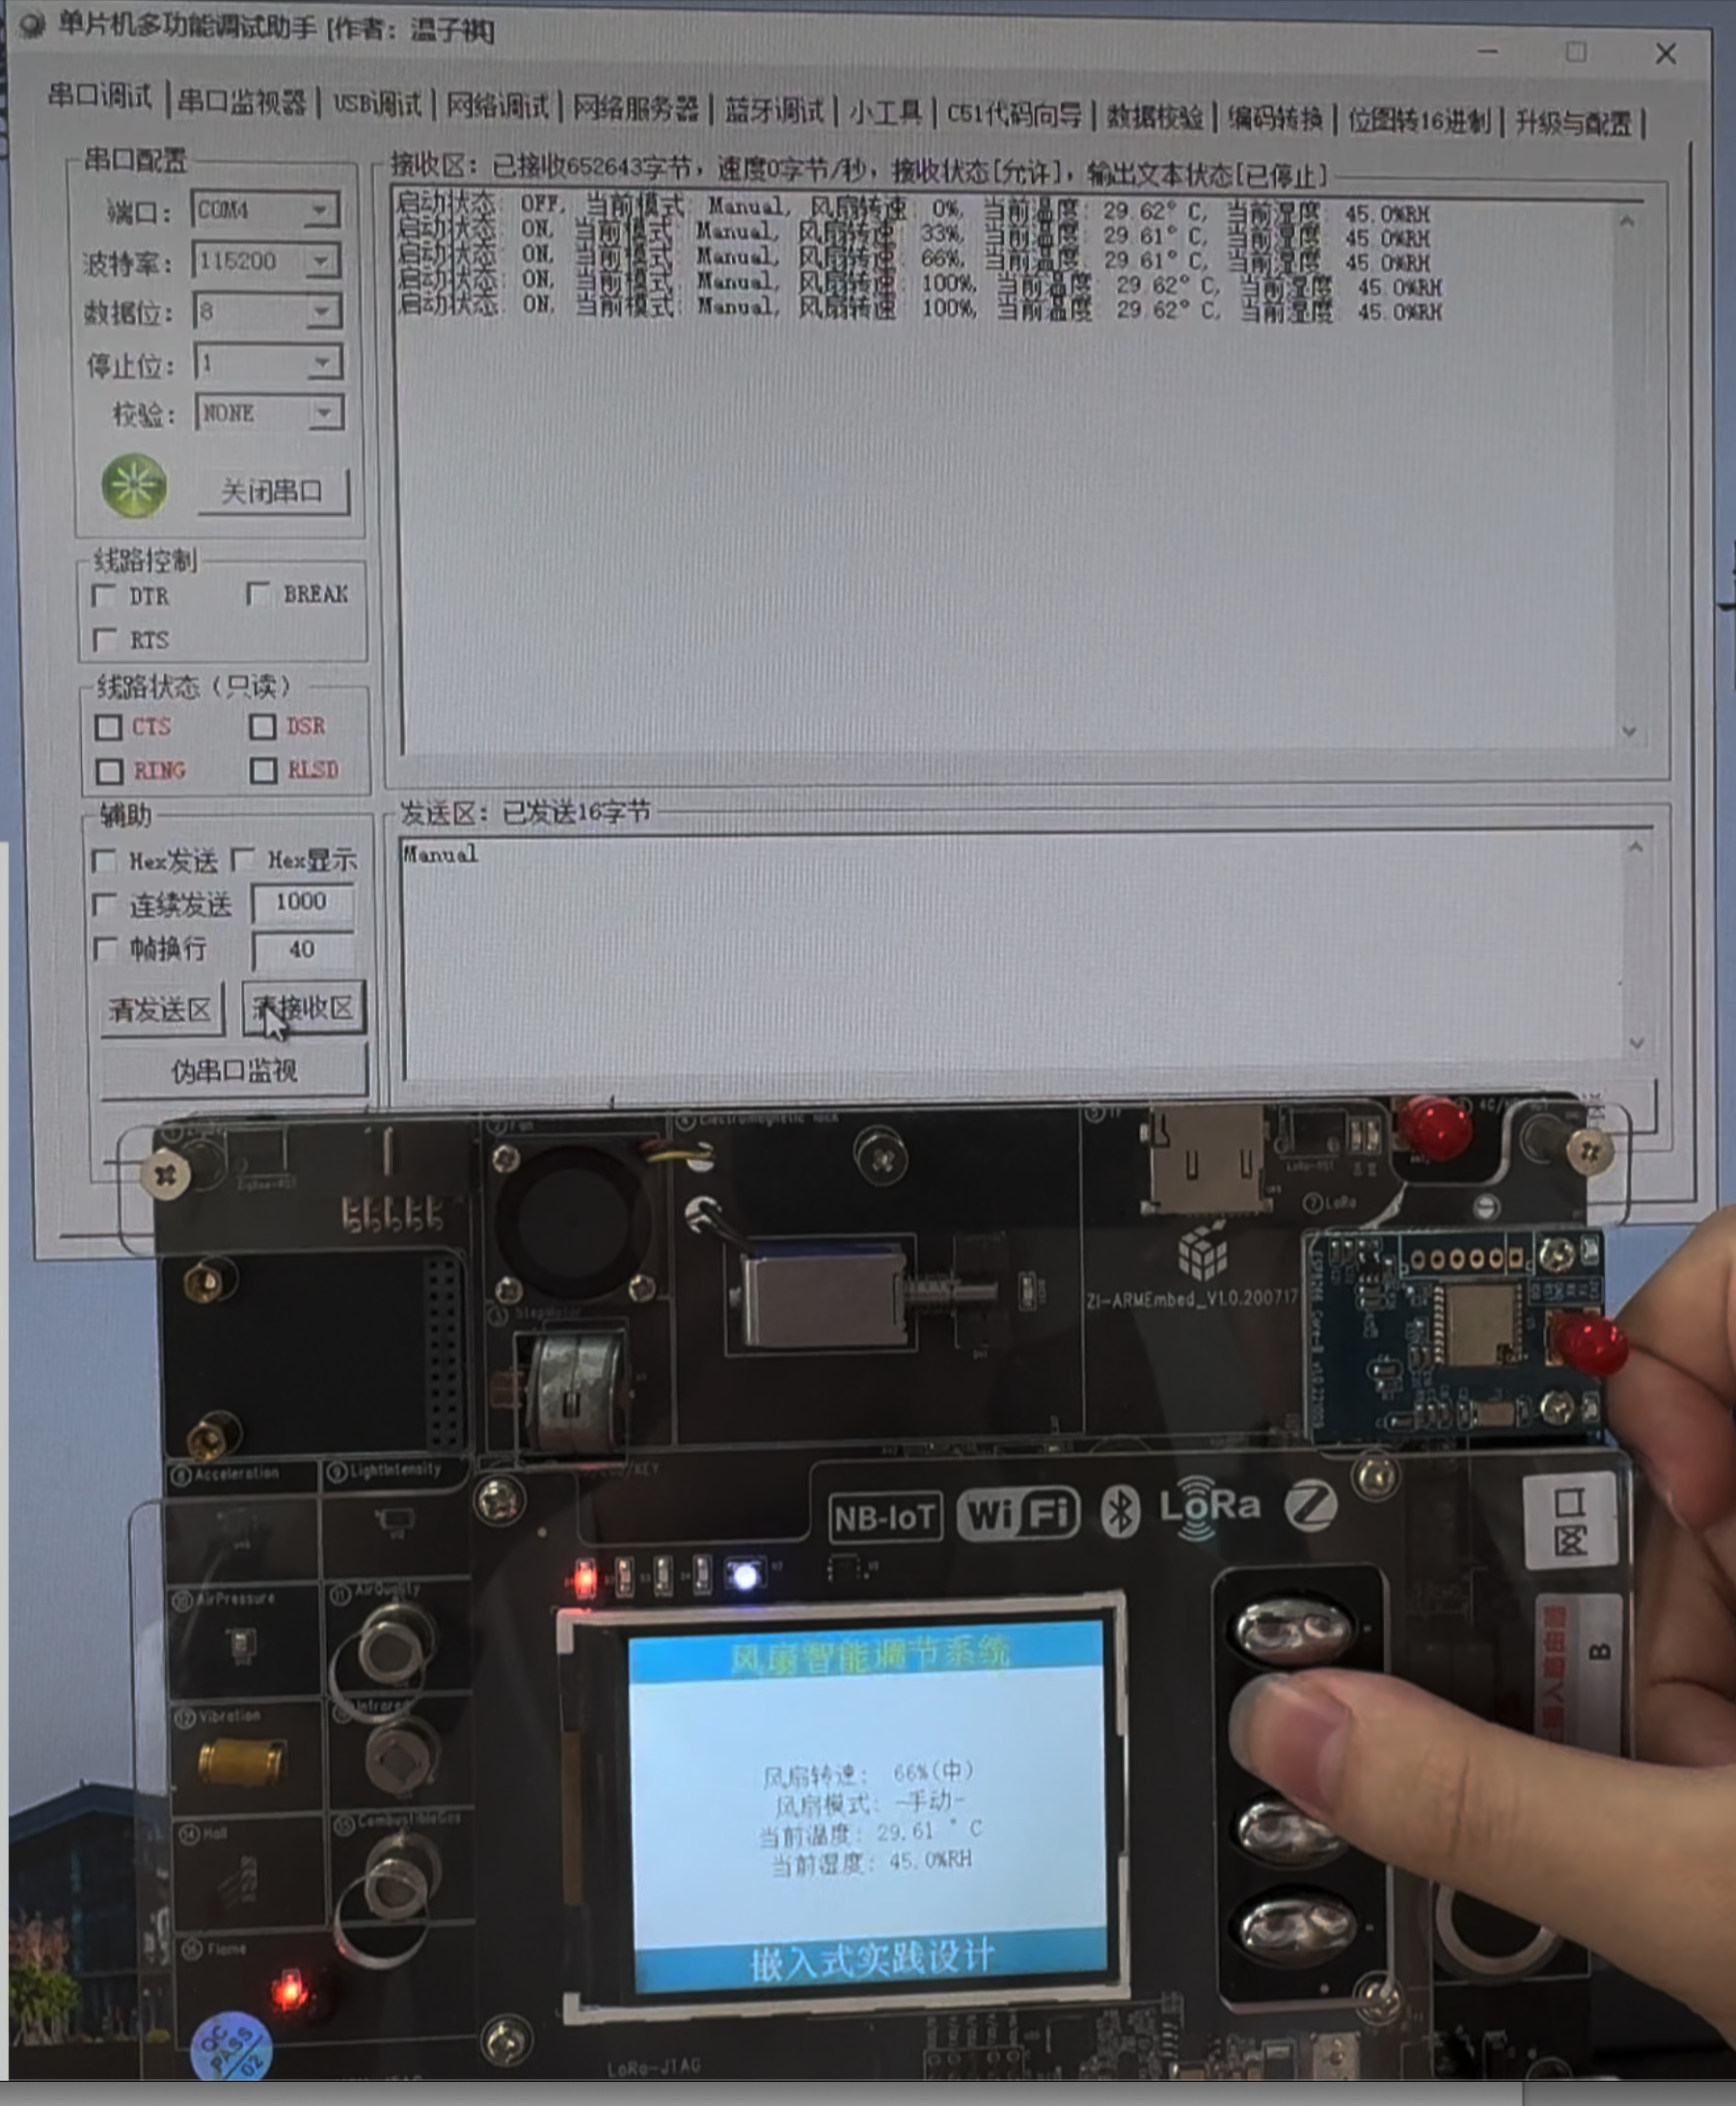
\includegraphics[width=0.45\textwidth]{../figures/CleanShot 2025-06-11 at 11.50.13@2x.png}
  \caption{温湿度检测功能调试结果}
  \label{fig:htu21d_debug}
\end{figure}

\subsubsection{风扇PWM控制功能调试}

\qquad 风扇控制是系统的核心执行功能,需要验证PWM输出、档位切换、转速精度等。

\textbf{调试内容:}
\begin{itemize}
    \vspace{-6pt}
  \item 验证PWM信号输出频率(50kHz)和占空比准确性
    \vspace{-6pt}
  \item 测试0档(0\%)、1档(33\%)、2档(66\%)、3档(100\%)四个档位
    \vspace{-6pt}
  \item 检查档位切换的平滑性和响应速度
    \vspace{-6pt}
  \item 确认风扇运行的稳定性和噪音水平
\end{itemize}

\textbf{调试方法:}使用示波器测量PWM信号,观察风扇转速变化,测试长时间运行稳定性。

\subsubsection{RGB LED状态指示功能调试}

\qquad RGB LED提供直观的系统状态指示,需要验证颜色控制、状态映射等功能。

\textbf{调试内容:}
\begin{itemize}
    \vspace{-6pt}
  \item 测试RGB LED的基本颜色显示功能
    \vspace{-6pt}
  \item 验证不同风扇档位对应的颜色指示
    \vspace{-6pt}
  \item 检查状态变化时LED的响应速度
    \vspace{-6pt}
  \item 确认LED亮度和颜色的视觉效果
\end{itemize}

\textbf{调试方法:}手动切换风扇档位,观察RGB LED颜色变化,验证状态指示的准确性和直观性。

% 预留图片位置
\begin{figure}[H]
  \centering
  \begin{subfigure}{0.45\textwidth}
    \centering
    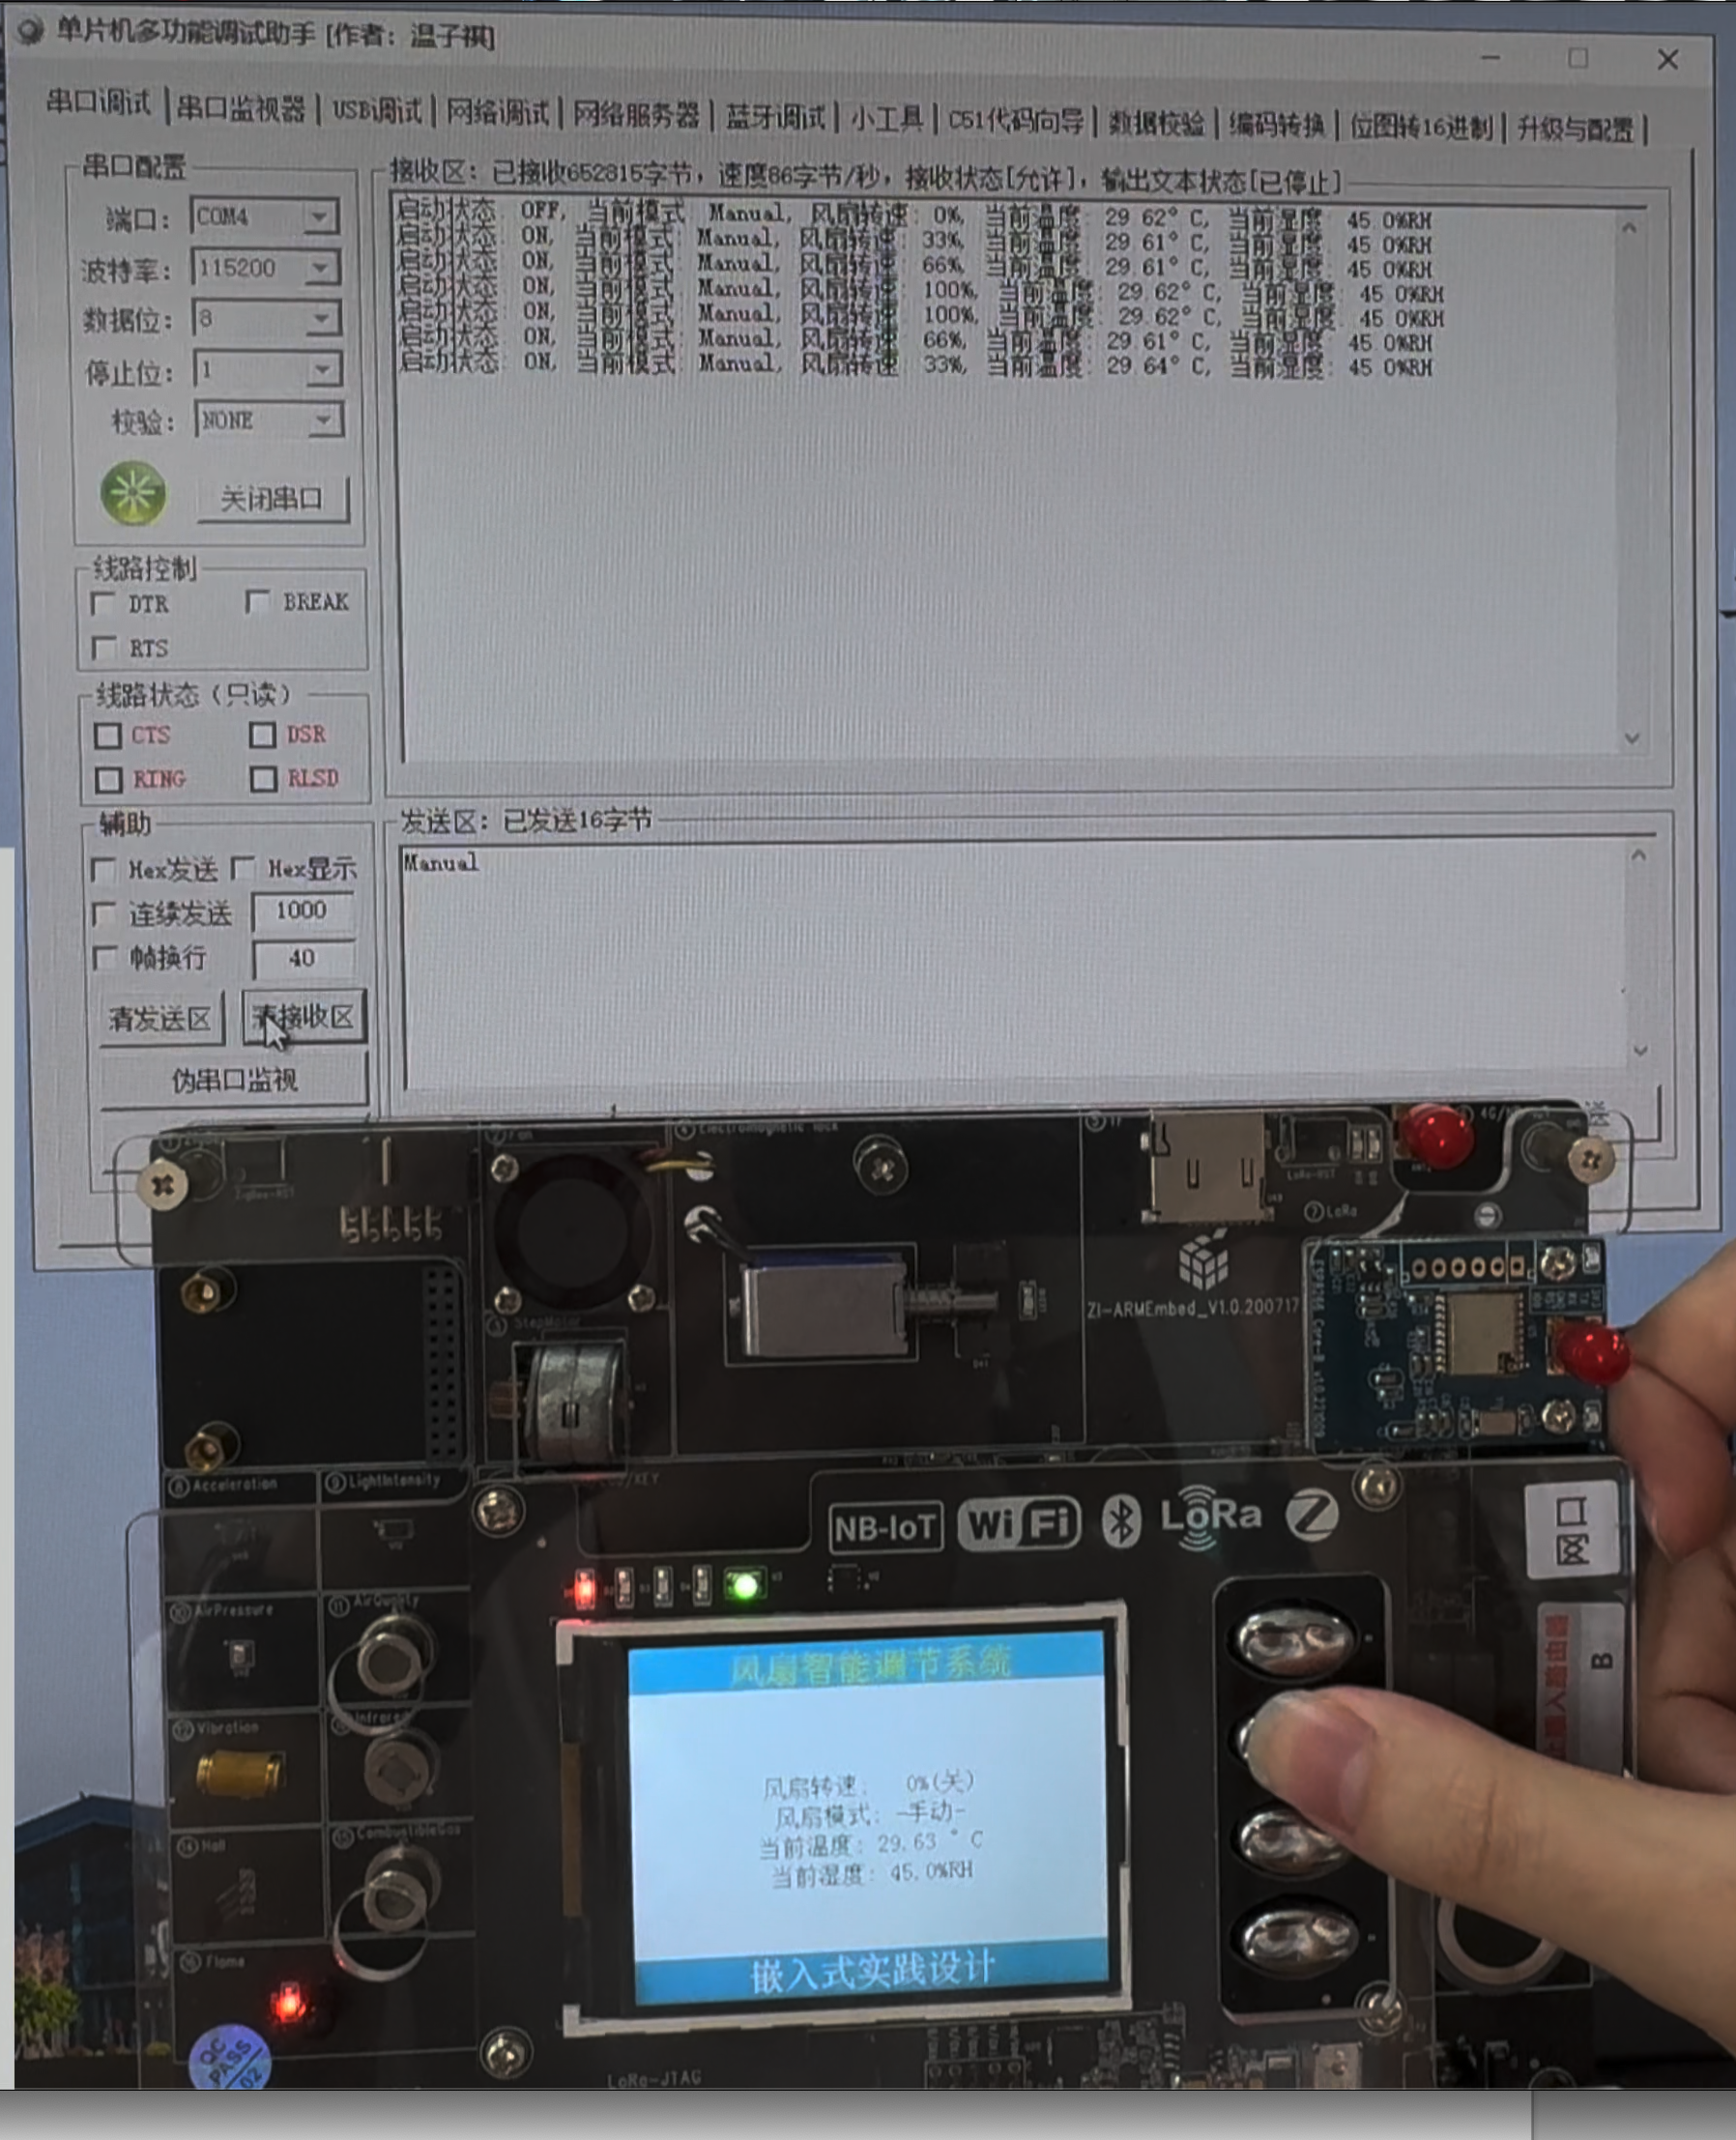
\includegraphics[width=\textwidth]{../figures/CleanShot 2025-06-11 at 11.53.10@2x.png}
    \caption{风扇关闭状态}
  \end{subfigure}
  \hfill
  \begin{subfigure}{0.45\textwidth}
    \centering
    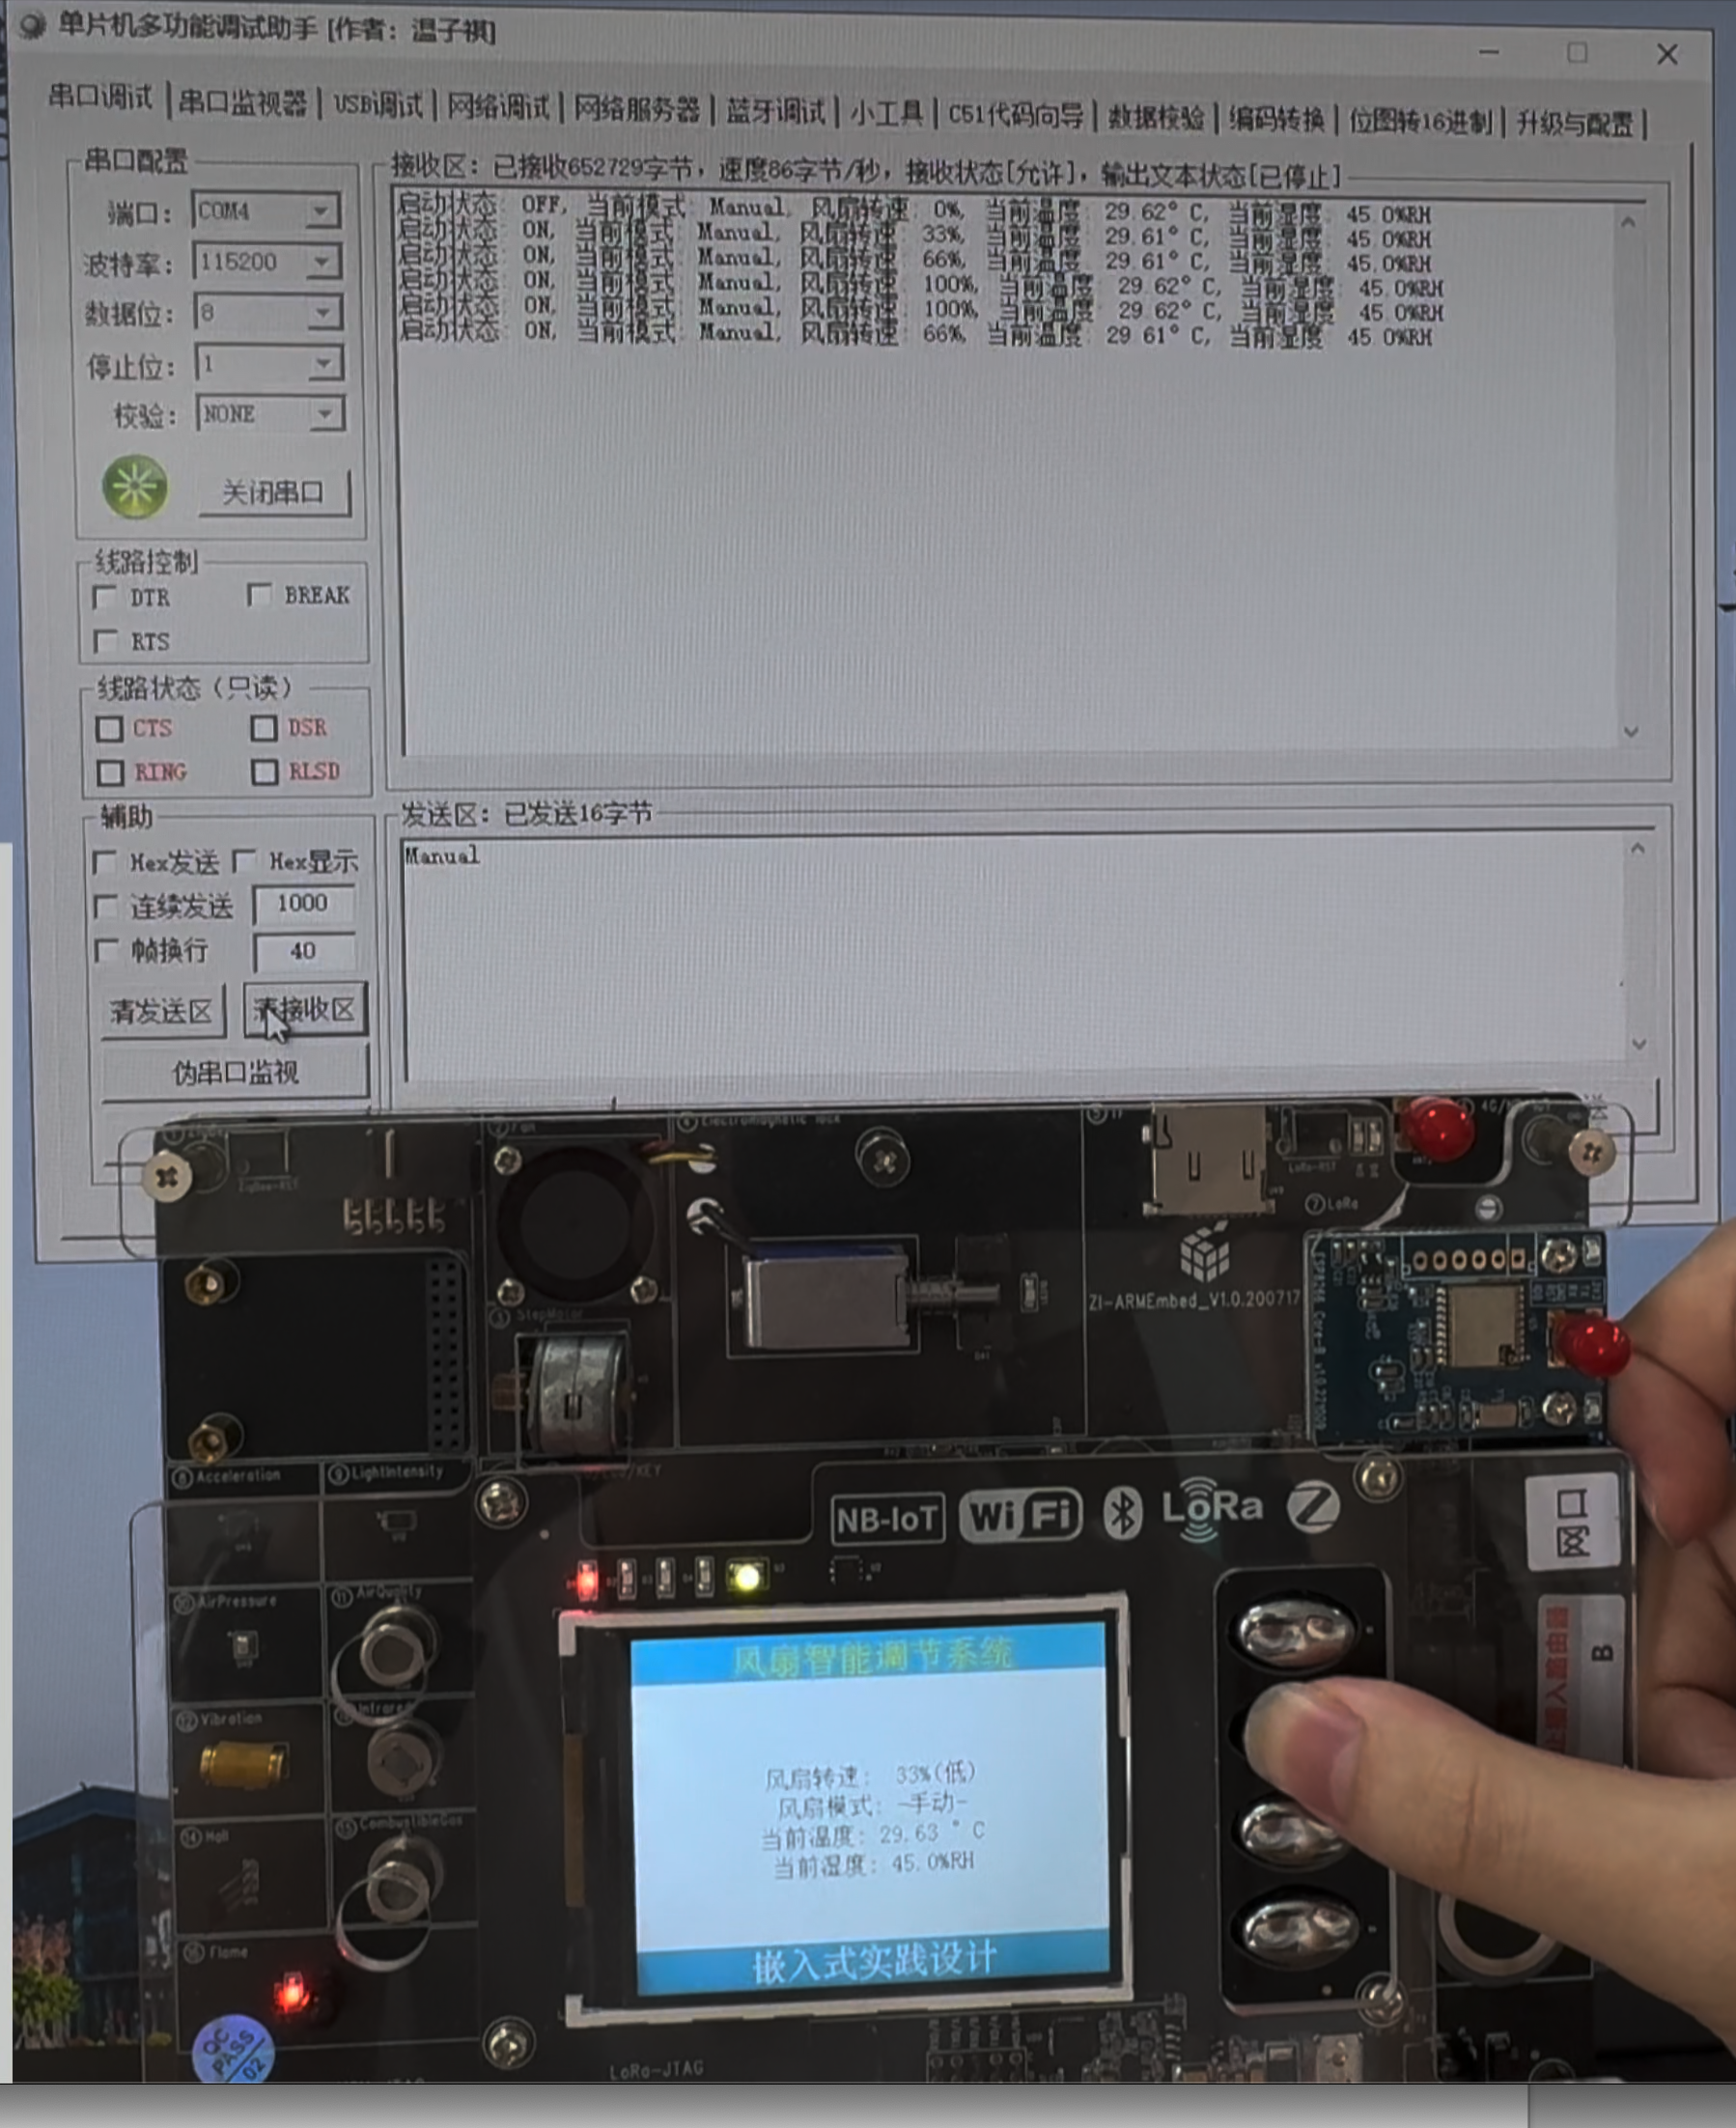
\includegraphics[width=\textwidth]{../figures/CleanShot 2025-06-11 at 11.52.57@2x.png}
    \caption{风扇转速33\%状态}
  \end{subfigure}

  \vspace{1pt}

  \centering
  \begin{subfigure}{0.45\textwidth}
    \centering
    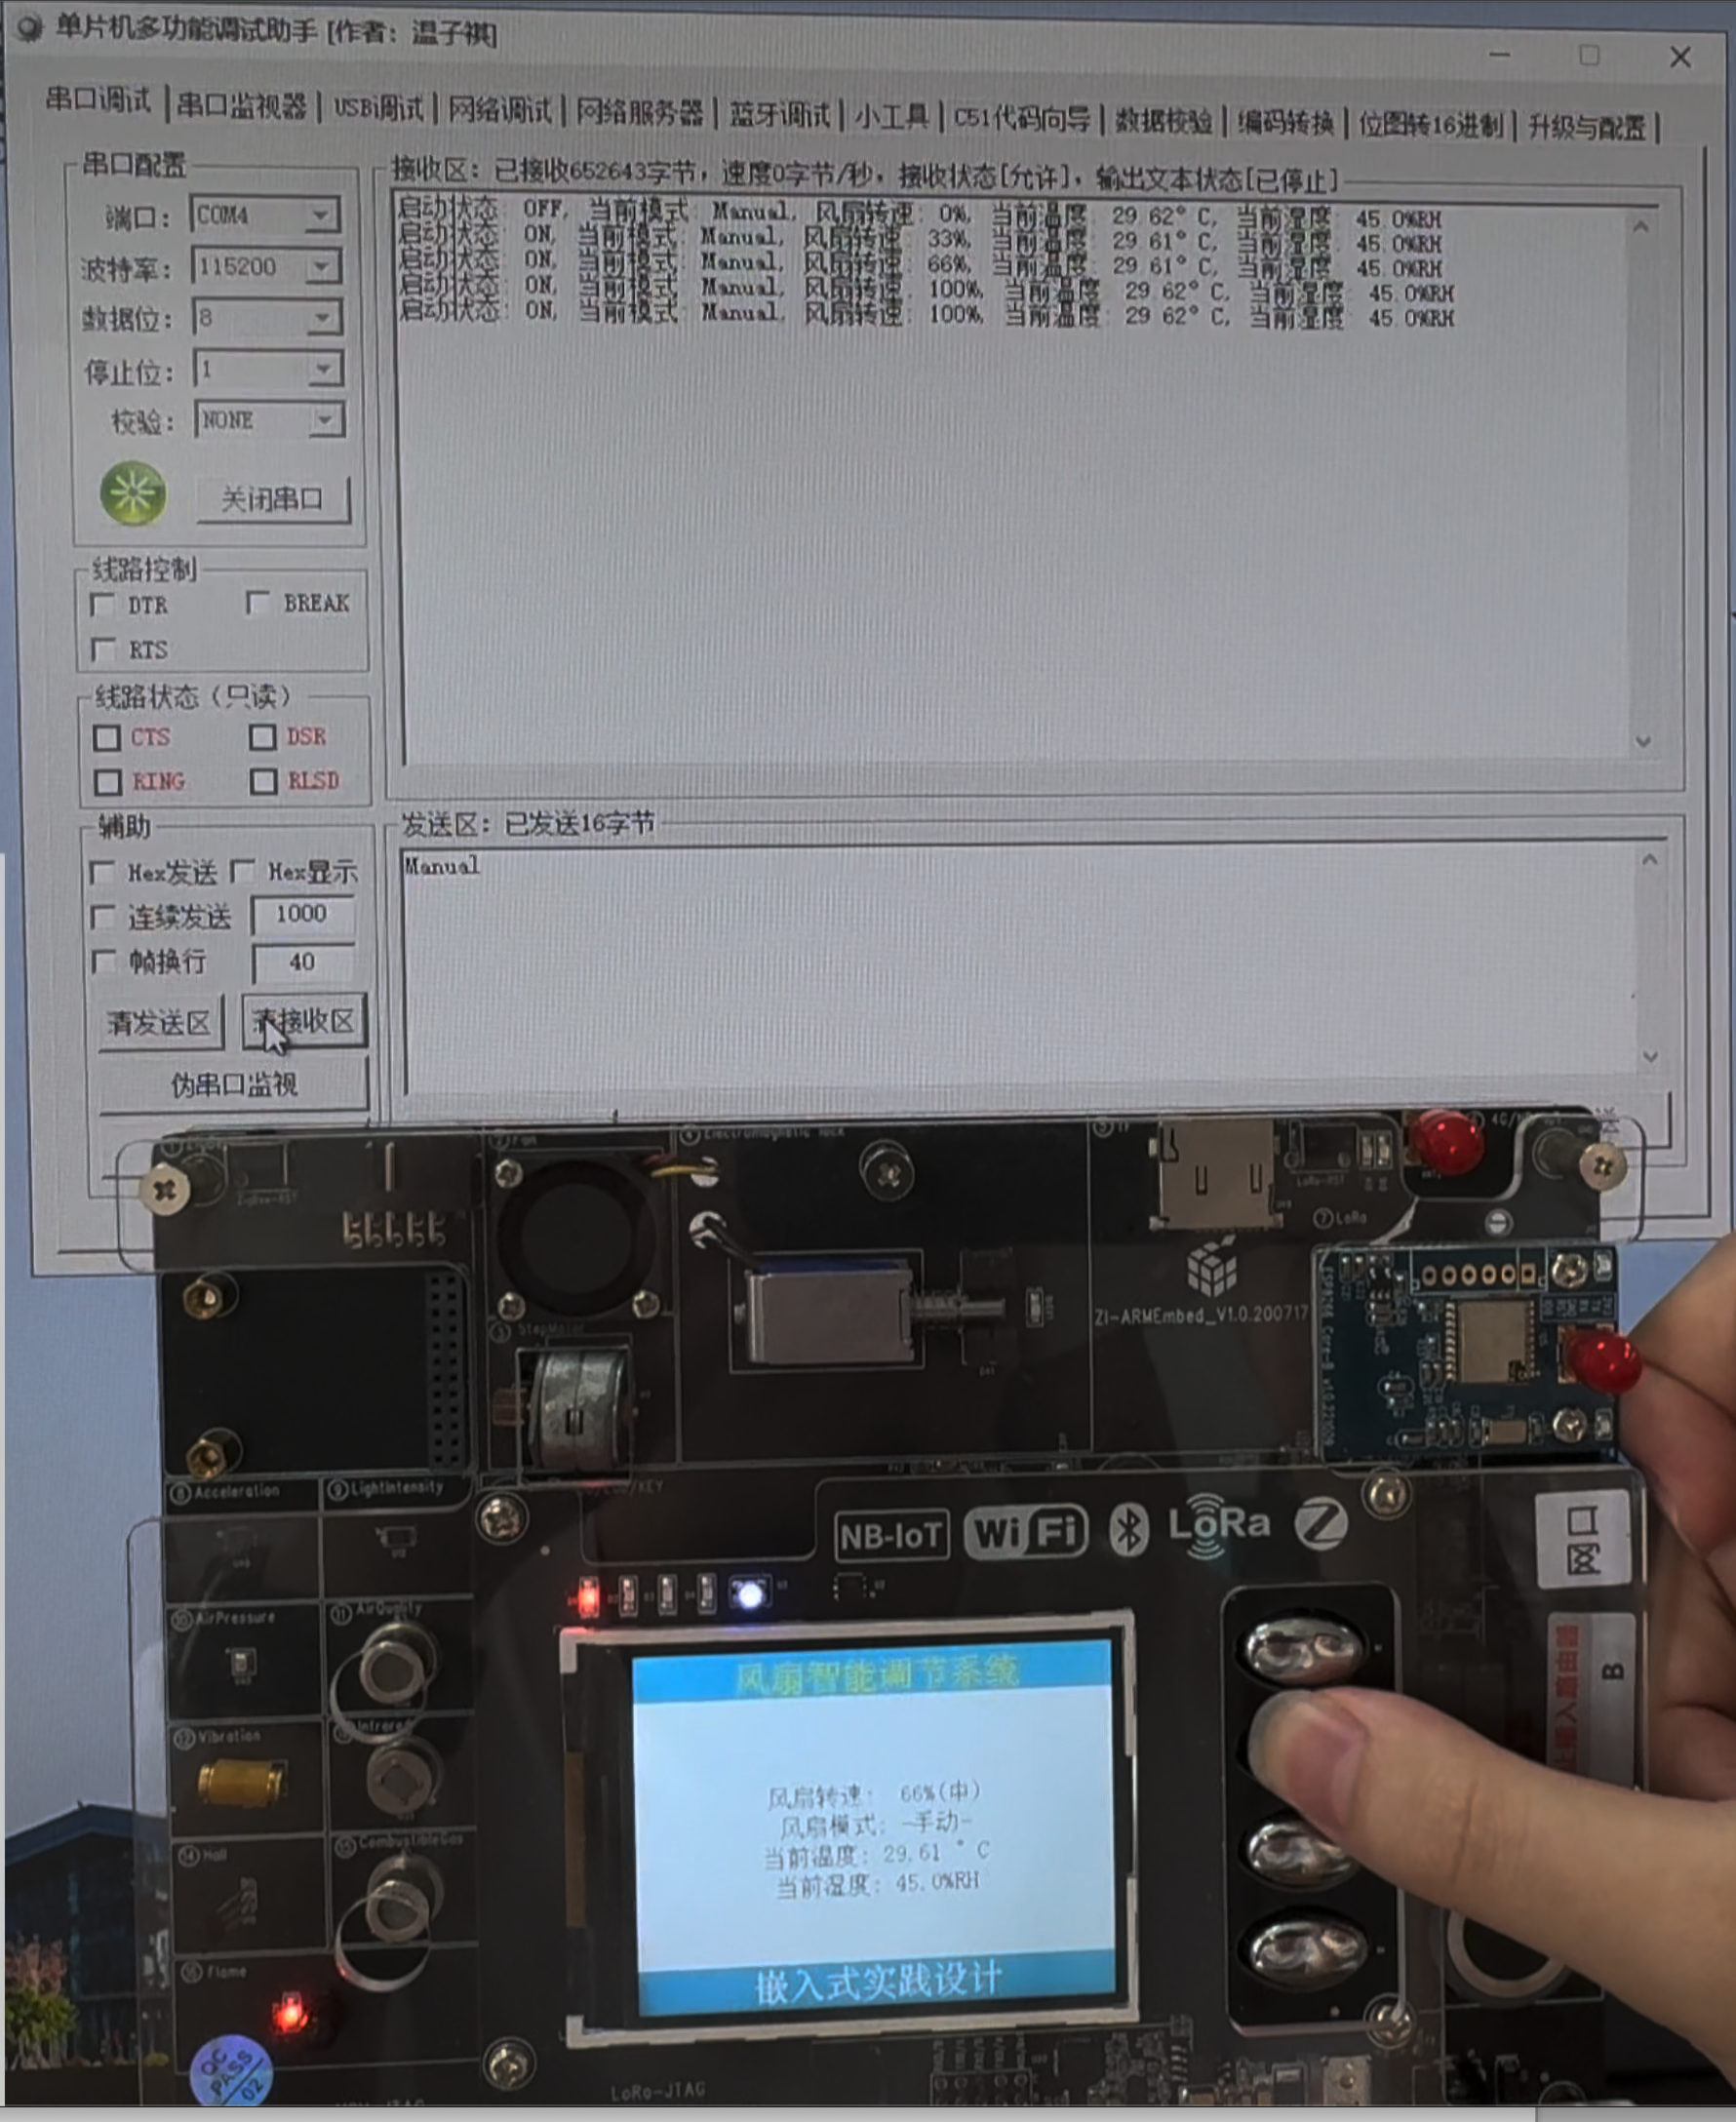
\includegraphics[width=\textwidth]{../figures/CleanShot 2025-06-11 at 11.52.44@2x.png}
    \caption{风扇转速66\%状态}
  \end{subfigure}
  \hfill
  \begin{subfigure}{0.45\textwidth}
    \centering
    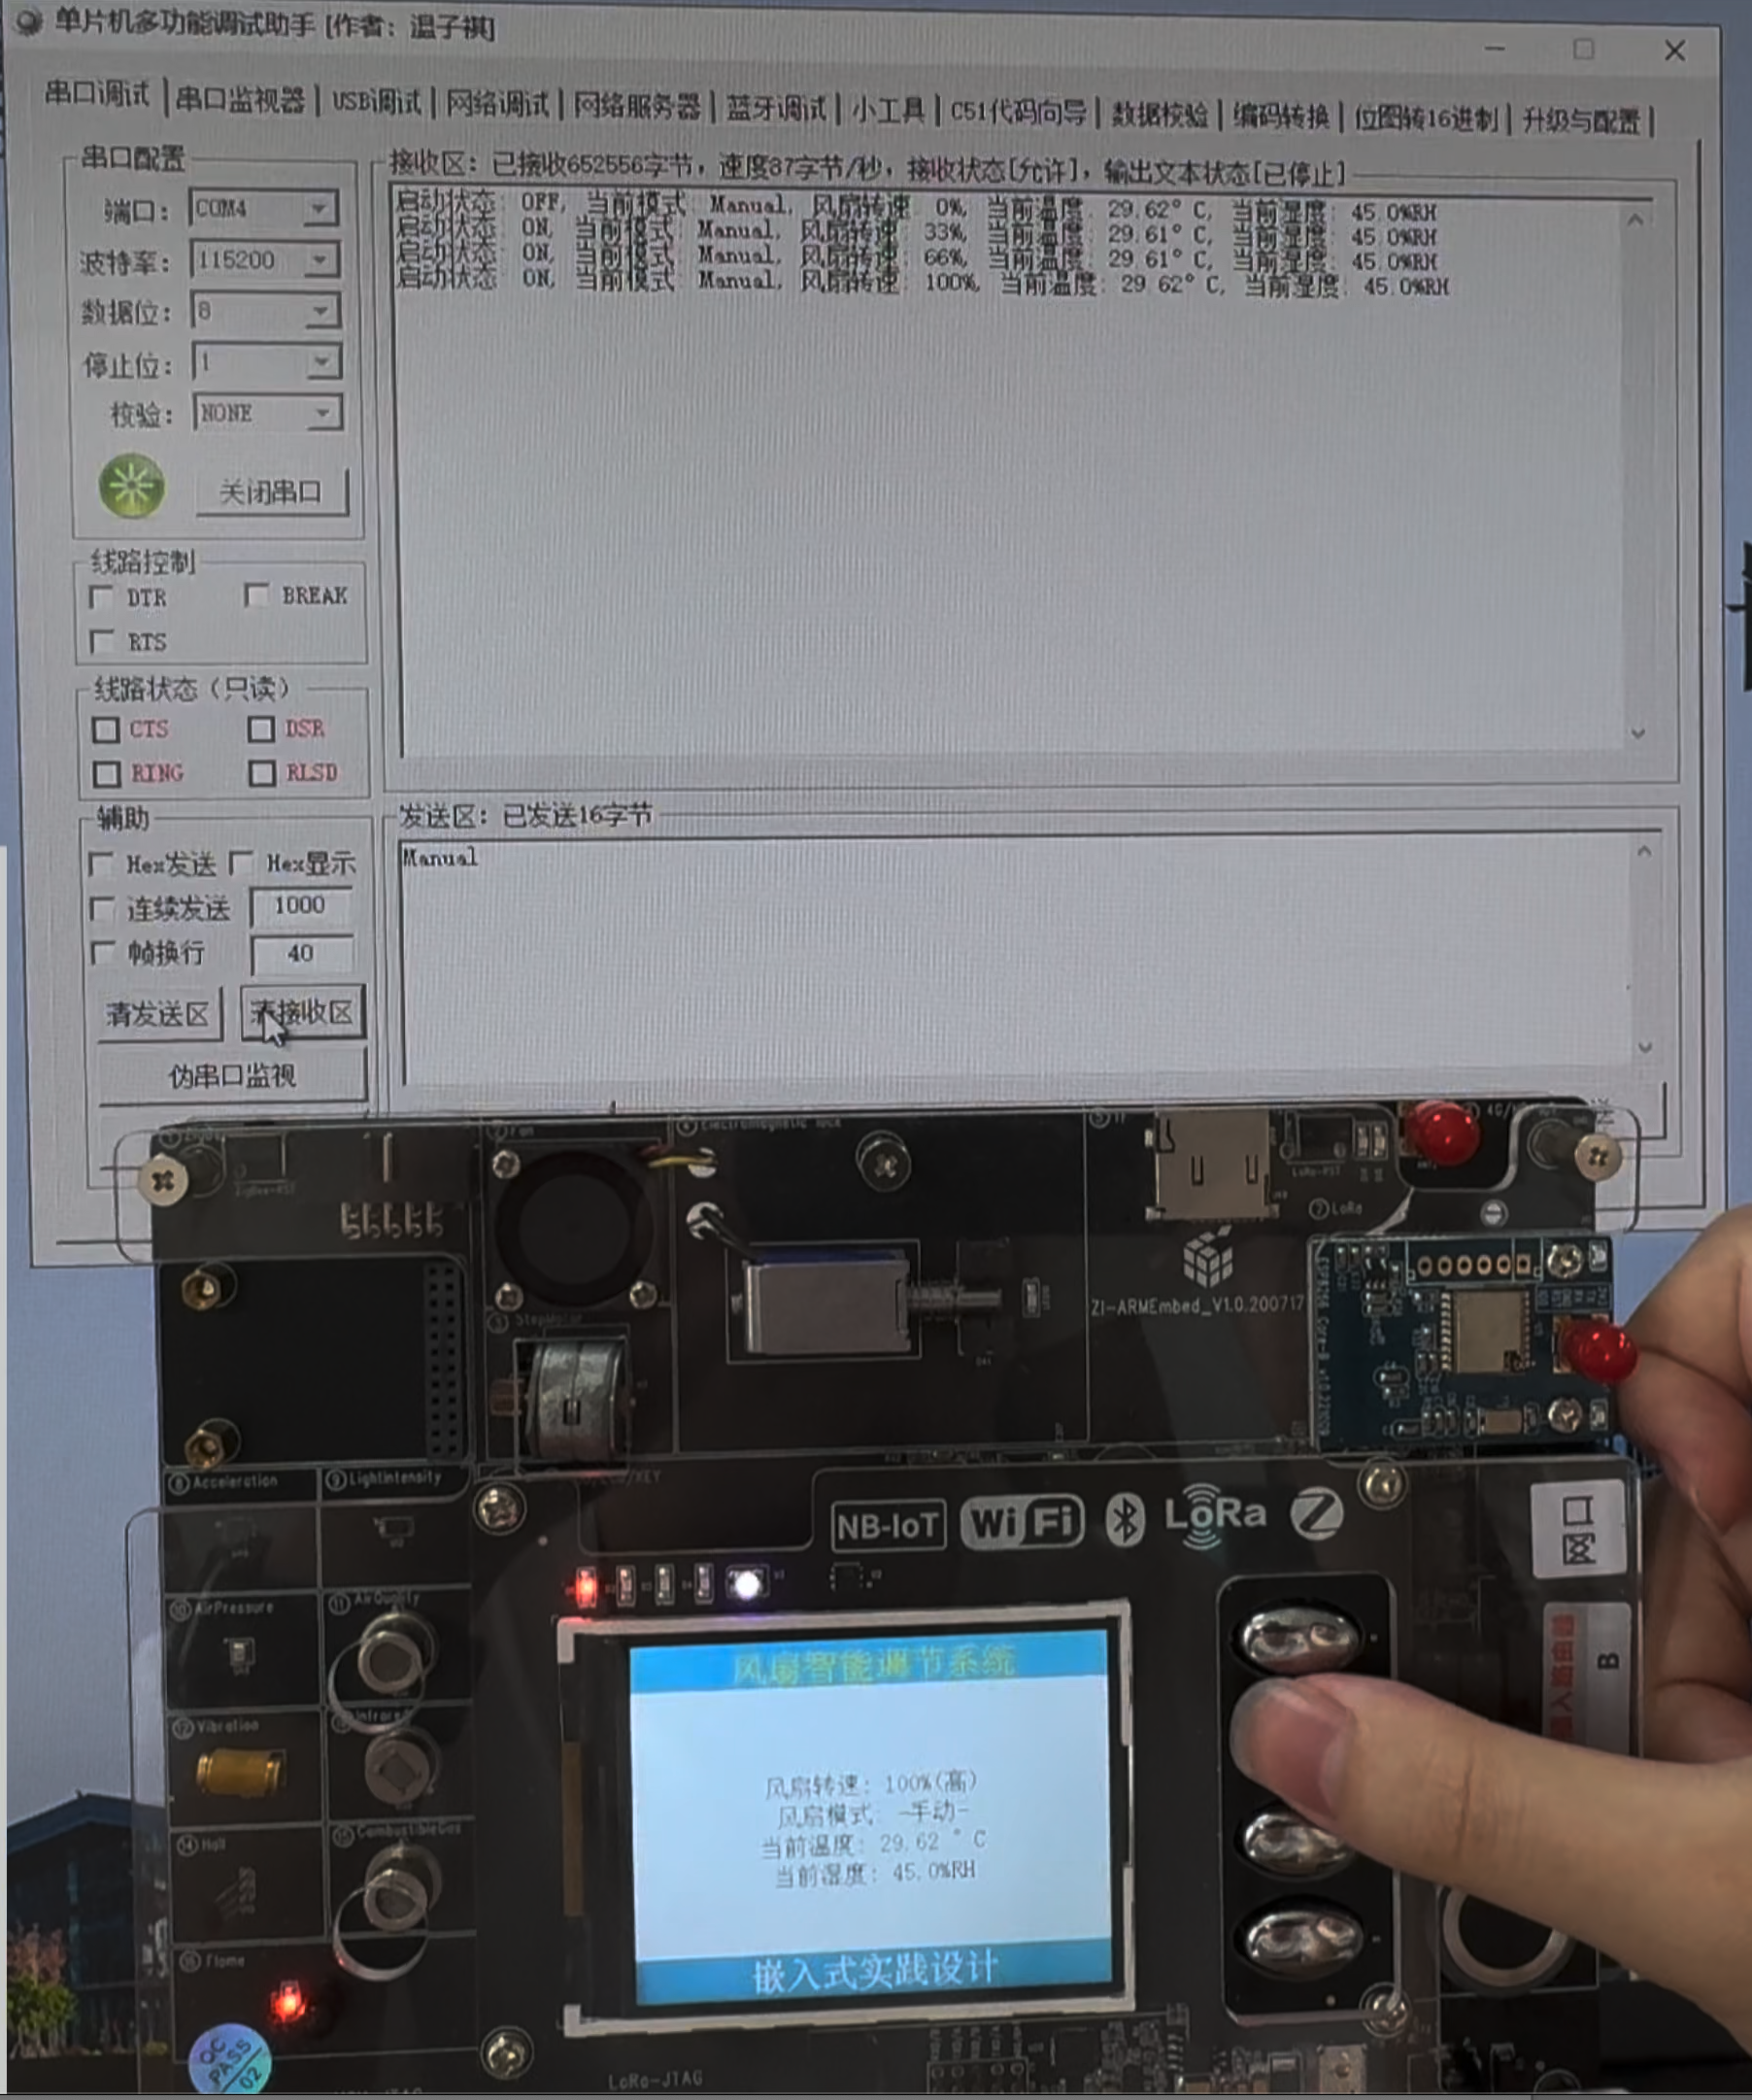
\includegraphics[width=\textwidth]{../figures/CleanShot 2025-06-11 at 11.52.25@2x.png}
    \caption{风扇转速100\%状态}
  \end{subfigure}

  \caption{RGB LED状态指示功能调试效果}
  \label{fig:rgb_led_debug}
\end{figure}

\subsubsection{蜂鸣器功能调试}

\qquad 蜂鸣器提供声音反馈,包括按键确认和高温报警等功能。

\textbf{调试内容:}
\begin{itemize}
    \vspace{-6pt}
  \item 测试蜂鸣器的基本发声功能
    \vspace{-6pt}
  \item 验证按键操作时的确认提示音
    \vspace{-6pt}
  \item 检查高温报警时的蜂鸣器响应(最多3次)
    \vspace{-6pt}
  \item 确认声音大小和持续时间的合理性
\end{itemize}

\textbf{调试方法:}通过按键操作和温度模拟测试蜂鸣器响应,验证报警机制的有效性。

\subsubsection{UART串口通信功能调试}

\qquad 串口通信实现远程控制和状态监测,是系统扩展性的重要保障。

\textbf{调试内容:}
\begin{itemize}
    \vspace{-6pt}
  \item 验证串口初始化配置(115200bps波特率)
    \vspace{-6pt}
  \item 测试"Auto"和"Manual"模式切换命令接收
    \vspace{-6pt}
  \item 检查系统状态信息的定时发送(每3ms)
    \vspace{-6pt}
  \item 确认数据传输的准确性和稳定性
\end{itemize}

\textbf{调试方法:}使用串口调试工具发送控制命令,监控系统状态输出,验证通信协议的正确性。

% 预留图片位置
\begin{figure}[H]
  \centering
  \begin{subfigure}{0.45\textwidth}
    \centering
    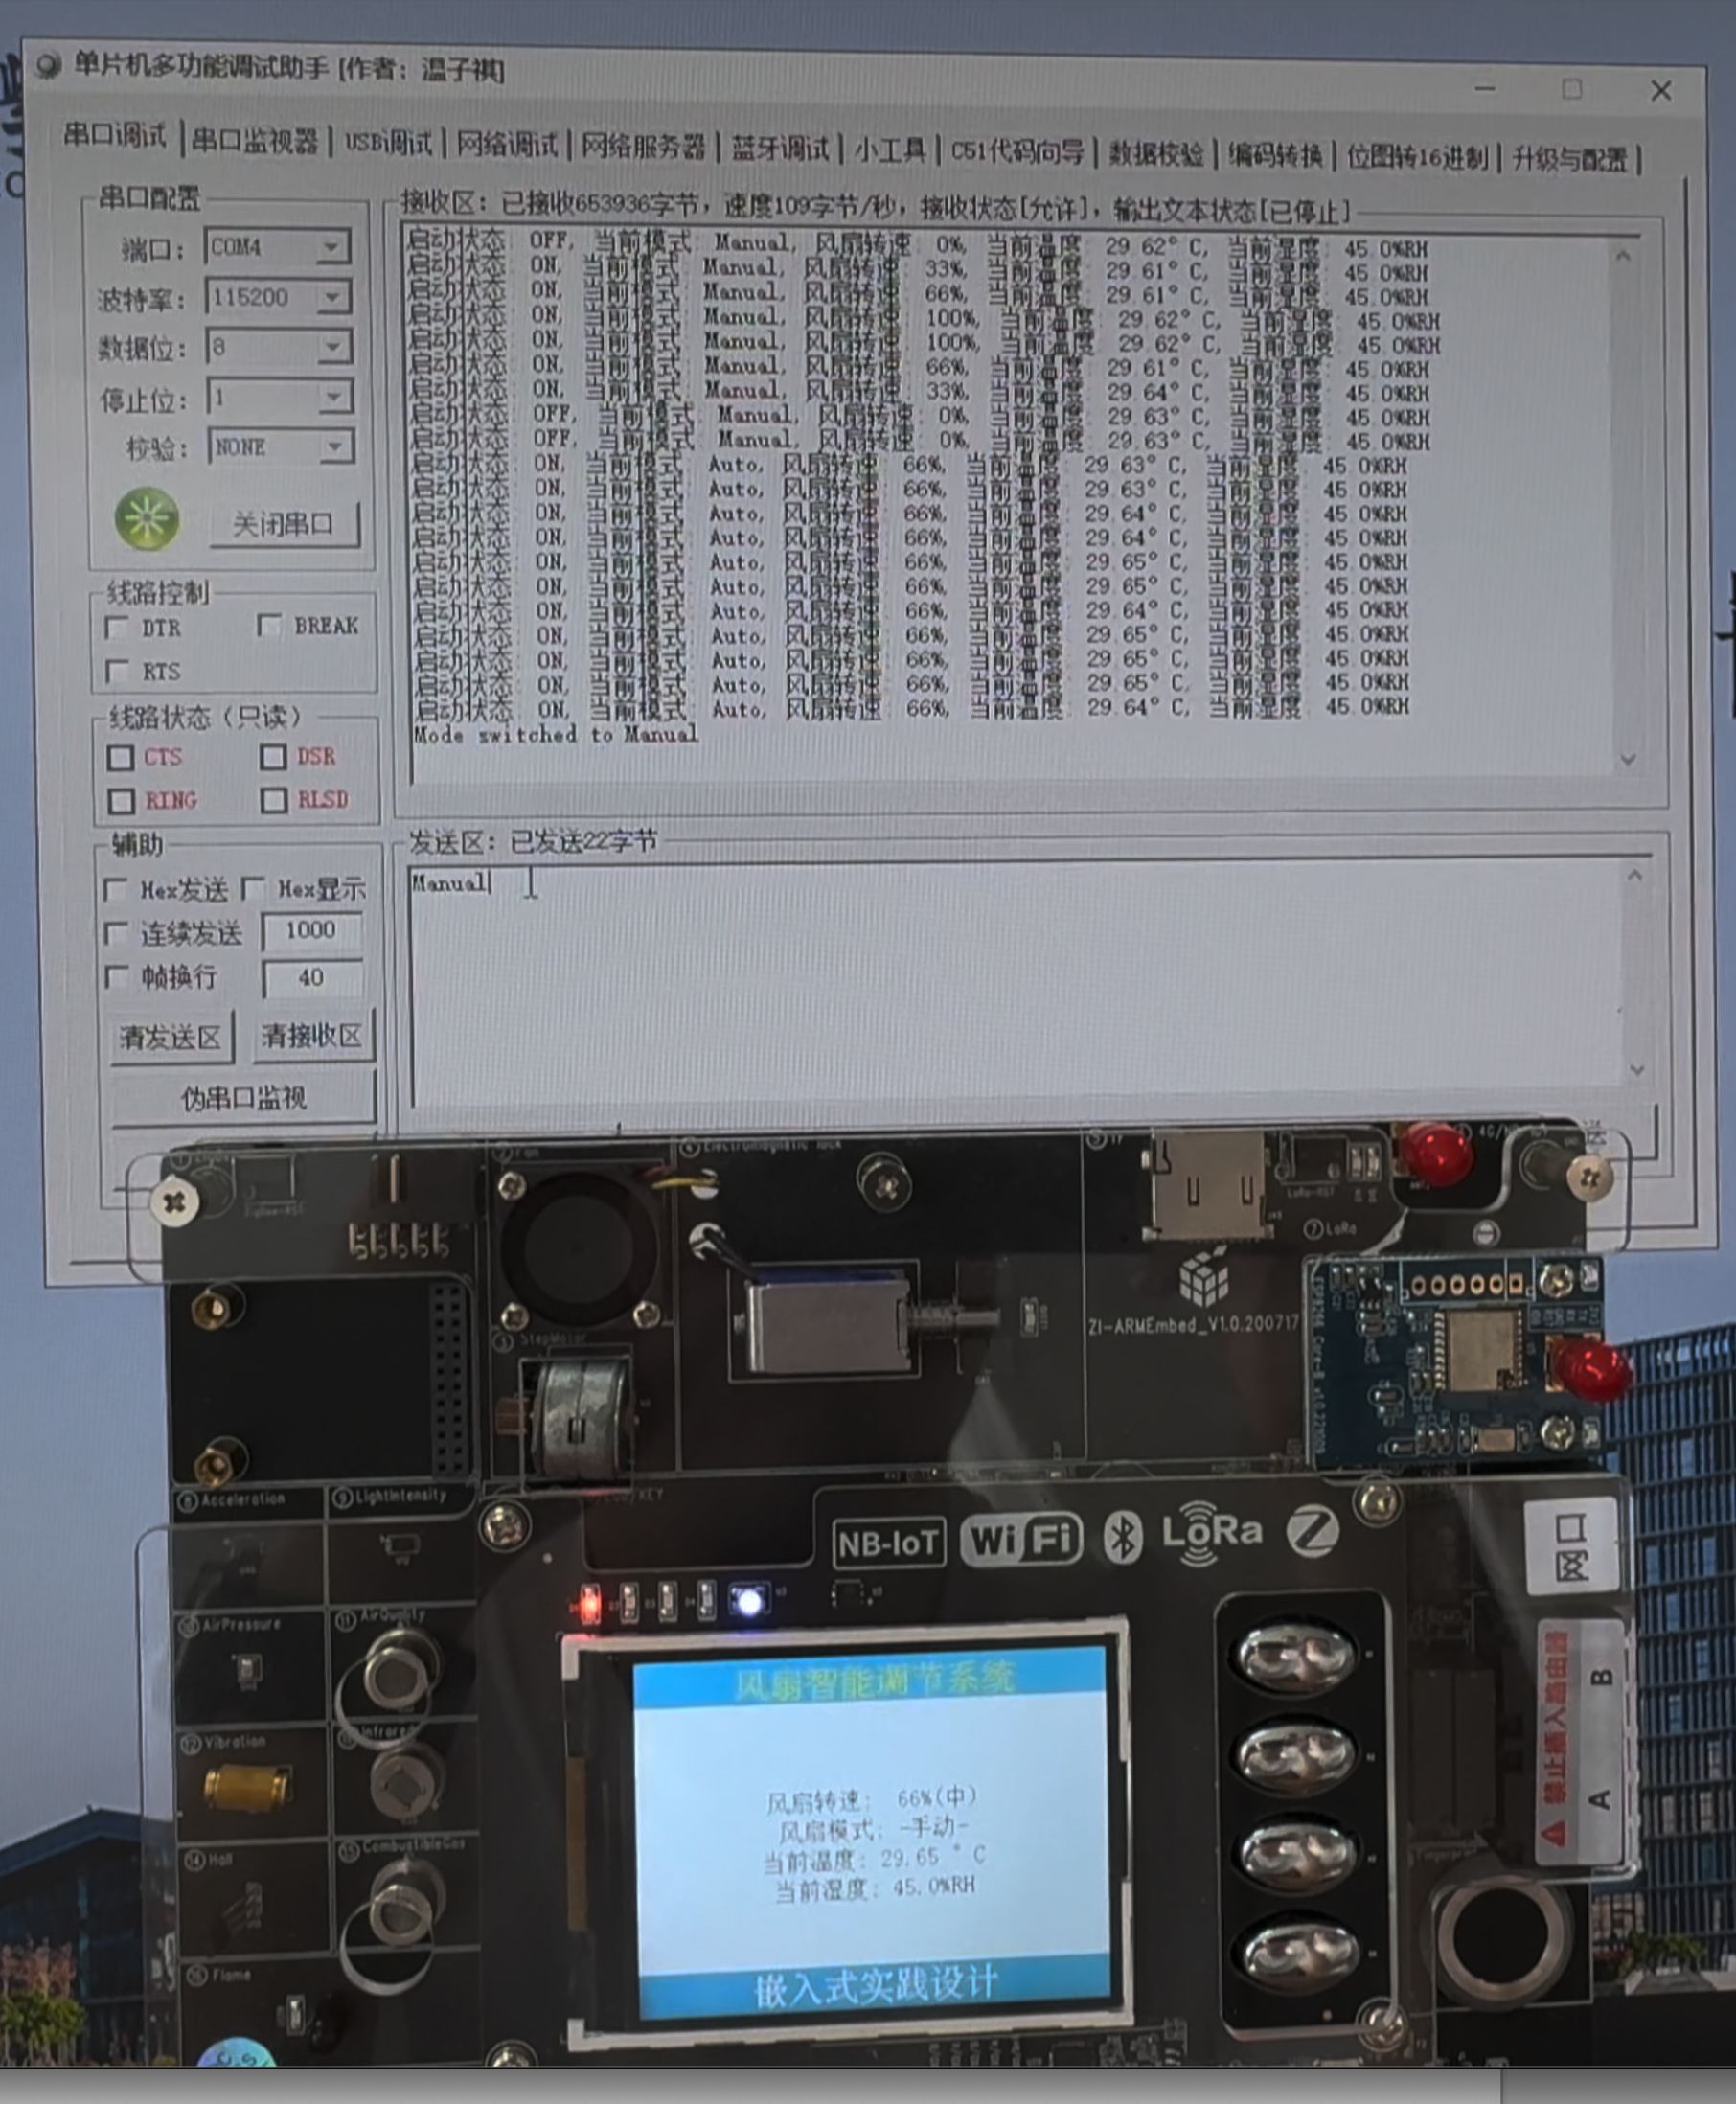
\includegraphics[width=\textwidth]{../figures/CleanShot 2025-06-11 at 12.03.40@2x.png}
    \caption{串口发送Manual状态}
  \end{subfigure}
  \hfil
  \begin{subfigure}{0.45\textwidth}
    \centering
    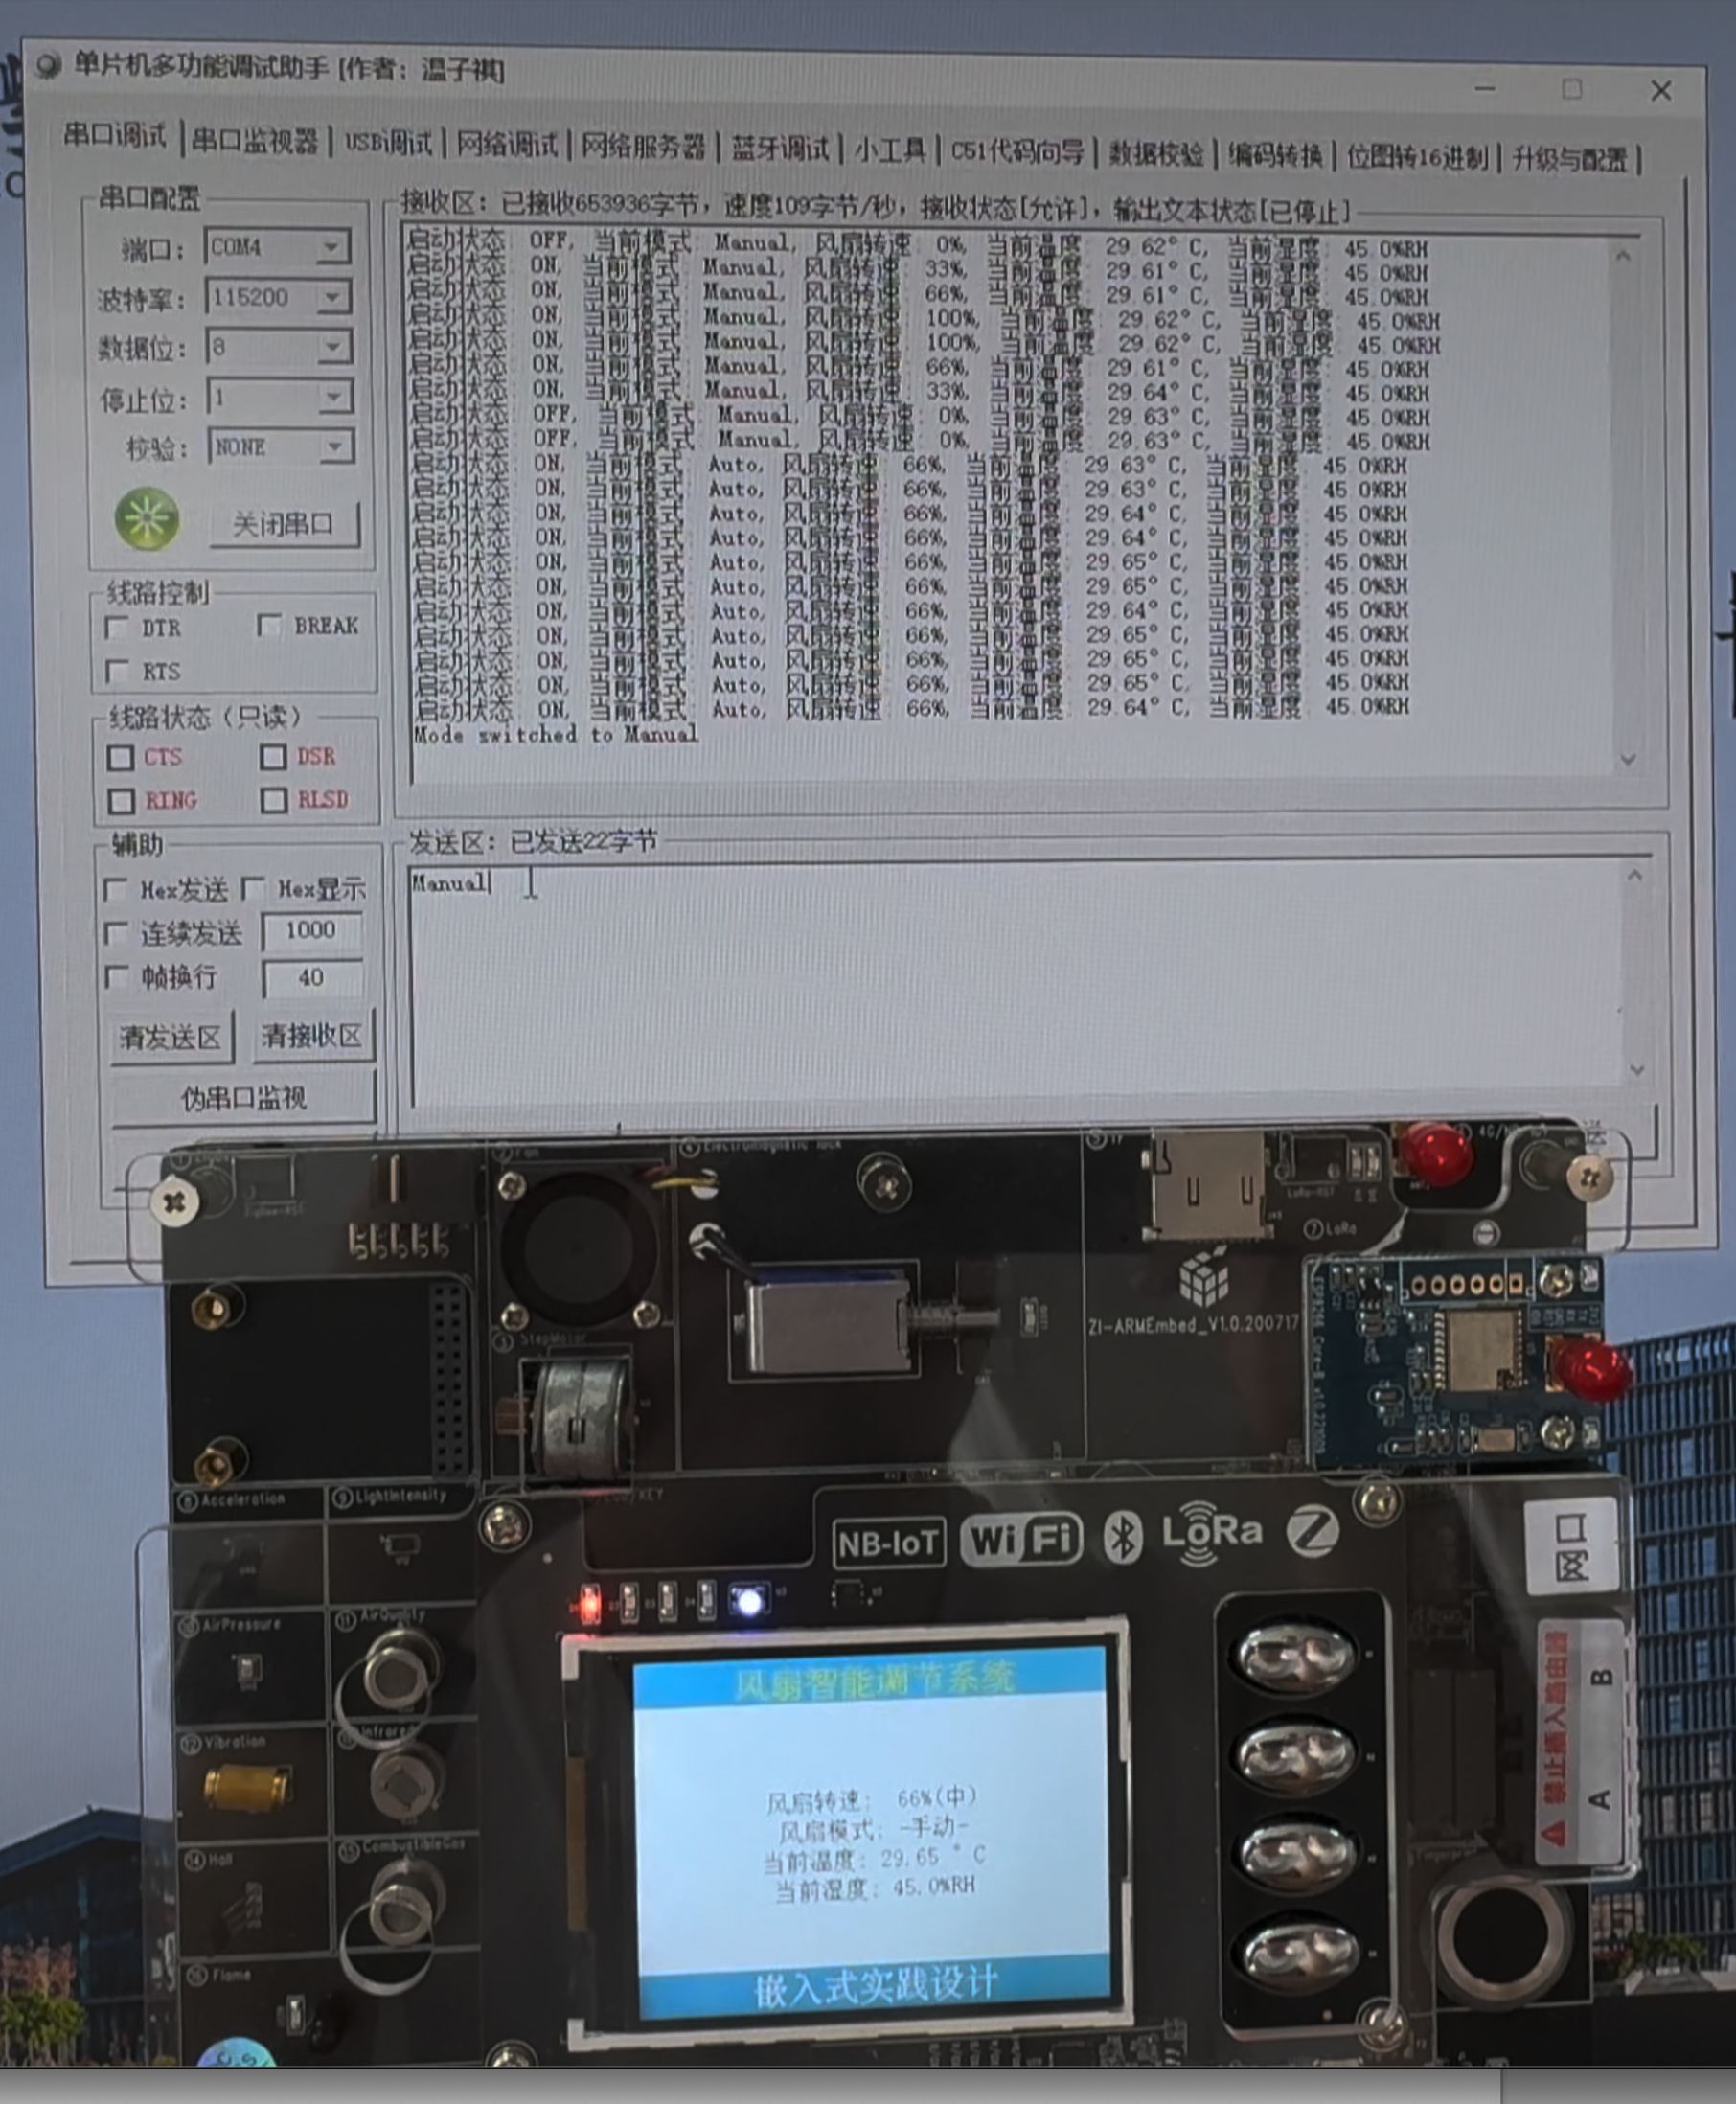
\includegraphics[width=\textwidth]{../figures/CleanShot 2025-06-11 at 12.03.40@2x.png}
    \caption{串口发送Auto状态}
  \end{subfigure}

  \caption{UART串口通信功能调试界面}
  \label{fig:uart_debug}
\end{figure}

\subsubsection{自动控制功能调试}

\qquad 自动控制是系统智能化的核心功能,需要验证温度阈值判断、自动档位调节等逻辑。

\textbf{调试内容:}
\begin{itemize}
    \vspace{-6pt}
  \item 测试温度阈值判断逻辑(20°C、25°C、30°C)
    \vspace{-6pt}
  \item 验证不同温度区间的自动档位切换
    \vspace{-6pt}
  \item 检查高温报警机制的触发条件
    \vspace{-6pt}
  \item 确认自动控制的响应速度和准确性
\end{itemize}

\textbf{调试方法:}通过温度模拟或环境温度变化测试自动控制逻辑,观察档位切换和状态指示。

% 预留图片位置
\begin{figure}[H]
  \centering
  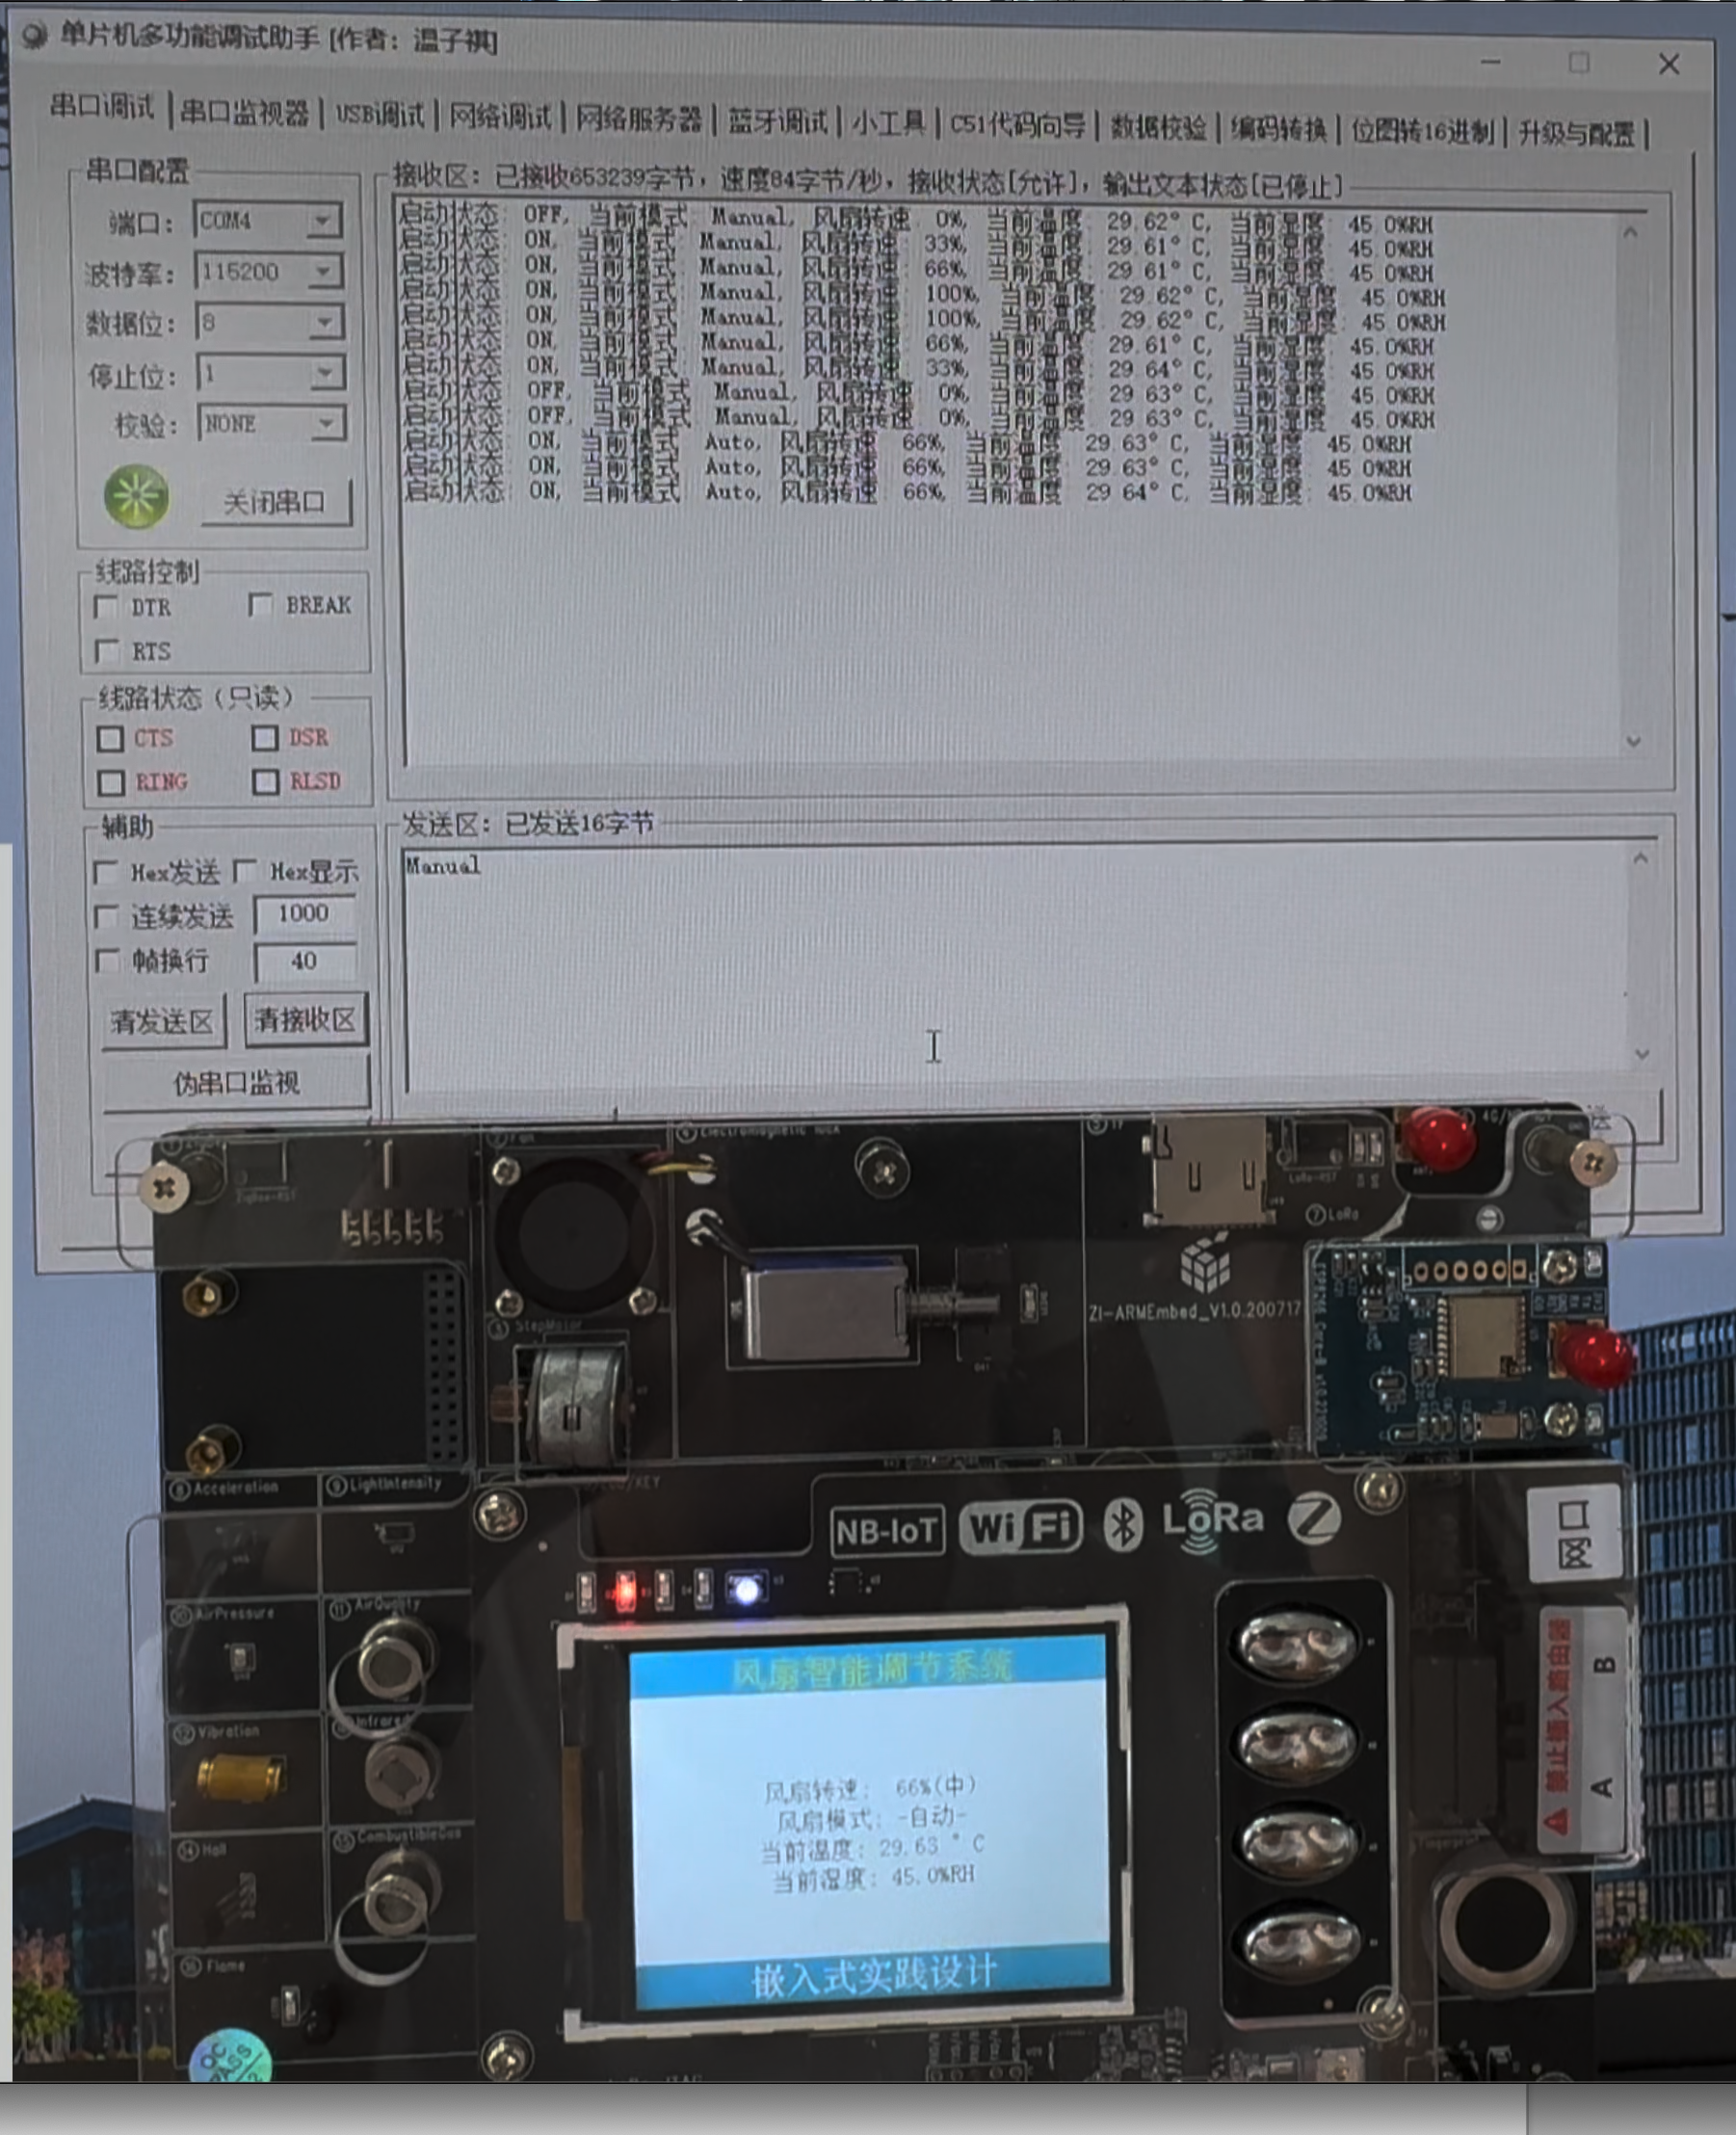
\includegraphics[width=0.45\textwidth]{../figures/CleanShot 2025-06-11 at 12.05.56@2x.png}
  \caption{自动控制功能调试过程}
  \label{fig:auto_control_debug}
\end{figure}

\subsubsection{手动控制功能调试}

\qquad 手动控制提供用户自主操作能力,需要验证按键响应、档位调节等功能。

\textbf{调试内容:}
\begin{itemize}
    \vspace{-6pt}
  \item 测试K1按键增加档位功能
    \vspace{-6pt}
  \item 验证K2按键减少档位功能
    \vspace{-6pt}
  \item 检查档位边界保护机制(0-3档)
    \vspace{-6pt}
  \item 确认手动模式下的状态指示正确性
\end{itemize}

\textbf{调试方法:}在手动模式下测试档位调节,验证边界条件处理和用户体验。

\subsubsection{系统开关功能调试}

\qquad 系统开关功能是基本的电源管理功能,需要验证状态切换、数据保持等。

\textbf{调试内容:}
\begin{itemize}
    \vspace{-6pt}
  \item 测试K4按键的系统开关功能
    \vspace{-6pt}
  \item 验证关机状态下的风扇停止运行
    \vspace{-6pt}
  \item 检查开机状态的功能恢复
    \vspace{-6pt}
  \item 确认状态监测功能在关机状态下的保持
\end{itemize}

\textbf{调试方法:}反复测试开关机功能,验证状态保存和恢复的正确性。


\subsection{性能分析}

\qquad 智能风扇控制系统的性能分析从系统瓶颈、资源利用率等多个维度进行评估,为后续优化提供数据支撑。

\subsubsection{性能瓶颈分析}

\textbf{主要性能瓶颈点:}

\textbf{1. 主循环频率过高}
\begin{lstlisting}
while(1) {
    // 主循环执行频率约1000Hz (1ms一次)
    delay_ms(1);
}
\end{lstlisting}

\qquad \textbf{问题分析:}1ms的主循环对MCU资源消耗较大,CPU占用率偏高。\textbf{优化建议:}调整为5-10ms,减少CPU占用率。

\textbf{2. LCD更新频率过高}
\begin{lstlisting}
if (no_motion_timer % 100 == 0) {
    update_display(current_temp, current_humi);  // 每100ms更新一次
}
\end{lstlisting}

\qquad \textbf{问题分析:}LCD更新是耗时操作,每100ms更新过于频繁。\textbf{优化建议:}改为500ms-1s更新一次。

\textbf{3. 温湿度传感器读取频率高}
\begin{lstlisting}
// 系统关闭时仍在读取
send_system_status(htu21d_t(), htu21d_h());  // 每3ms执行一次
\end{lstlisting}

\qquad \textbf{问题分析:}I2C通信耗时,频繁读取影响响应速度。\textbf{优化建议:}缓存数据,降低读取频率。

\textbf{4. 字符串处理开销}
\begin{lstlisting}
int get_centered_x(const char *text) {
    // 每次LCD显示都要计算,包含循环遍历
    for (int i = 0; i < text_len; i++) { ... }
}
\end{lstlisting}

\qquad \textbf{问题分析:}每次显示都重新计算居中位置。\textbf{优化建议:}预计算常用字符串的居中位置。

\subsubsection{性能评估结果}

\begin{table}[H]
  \centering
  \caption{系统性能评估对比表}
  \label{tab:performance_evaluation}
  \begin{tabular}{|c|c|c|c|}
    \hline
    \textbf{性能指标} & \textbf{当前状态} & \textbf{优化目标} & \textbf{改进方案} \\
    \hline
    主循环频率 & 1000Hz & 100Hz & 调整延时为10ms \\
    \hline
    LCD更新频率 & 10Hz & 2Hz & 500ms更新一次 \\
    \hline
    按键响应时间 & 50ms & 10ms & 减少防抖延时 \\
    \hline
    温度读取频率 & 333Hz & 10Hz & 缓存传感器数据 \\
    \hline
    内存使用率 & 中等 & 低 & 优化字符串处理 \\
    \hline
    CPU占用率 & 高 & 中 & 降低循环频率 \\
    \hline
  \end{tabular}
\end{table}

\textbf{优点:}功能完整、逻辑清晰、模块化程度高

\textbf{改进点:}降低循环频率、优化I/O操作频率、减少字符串处理开销

\subsubsection{系统架构性能分析}

\textbf{核心模块组成及性能特征:}

\begin{itemize}
    \vspace{-6pt}
  \item \textbf{系统初始化模块} - 一次性执行,性能影响小
    \vspace{-6pt}
  \item \textbf{按键控制模块} - 中断驱动,响应速度快
    \vspace{-6pt}
  \item \textbf{温湿度监测模块} - I2C通信,存在性能瓶颈
    \vspace{-6pt}
  \item \textbf{风扇控制模块} - PWM硬件输出,性能优秀
    \vspace{-6pt}
  \item \textbf{LCD显示模块} - 刷新频繁,需要优化
    \vspace{-6pt}
  \item \textbf{UART通信模块} - 串口硬件支持,性能良好
\end{itemize}


\section{总结}

\subsection{项目完成情况}

\qquad 本项目成功完成了基于STM32F4xx微控制器的智能风扇控制系统的设计与实现。项目从需求分析、方案设计、软硬件实现到调试验证,全面达成了预期目标,实现了一个功能完整、性能稳定的智能控制系统。

\subsubsection{核心功能实现}

\textbf{1. 智能温控功能}
\begin{itemize}
    \vspace{-6pt}
  \item 成功集成HTU21D温湿度传感器,实现±0.3°C精度的温度检测
    \vspace{-6pt}
  \item 实现了基于温度阈值的四档自动控制:舒适区(<20°C)关闭、低温区(20-24°C)1档、中温区(25-29°C)2档、高温区(≥30°C)3档运行
    \vspace{-6pt}
  \item 集成高温报警机制,超温时蜂鸣器自动报警,最多响3次
\end{itemize}

\textbf{2. 多模式控制功能}
\begin{itemize}
    \vspace{-6pt}
  \item 实现自动/手动双模式切换,满足不同使用场景需求
    \vspace{-6pt}
  \item 手动模式支持0-3档位精确调节,对应PWM占空比0\%、33\%、66\%、100\%
    \vspace{-6pt}
  \item 支持UART串口远程控制,接收"Auto"和"Manual"命令切换模式
\end{itemize}

\textbf{3. 人机交互功能}
\begin{itemize}
    \vspace{-6pt}
  \item 320×240像素LCD实时显示系统状态、温湿度数据、工作模式等信息
    \vspace{-6pt}
  \item 实现中英文混合显示和智能居中对齐算法
    \vspace{-6pt}
  \item K1-K4四键操控:档位增减、模式切换、系统开关
    \vspace{-6pt}
  \item RGB LED状态指示和蜂鸣器声音反馈,提供直观操作体验
\end{itemize}

\subsubsection{技术指标达成}

\begin{table}[H]
  \centering
  \caption{系统技术指标完成情况对比表}
  \label{tab:technical_achievements}
  \begin{tabular}{|l|c|c|c|}
    \hline
    \textbf{技术指标} & \textbf{设计要求} & \textbf{实际实现} & \textbf{达成状态} \\
    \hline
    按键响应时间 & ≤50ms & 50ms(防抖) & ✓ 达成 \\
    \hline
    温度检测频率 & ≥10Hz & 实时检测 & ✓ 超额完成 \\
    \hline
    温度测量精度 & ±0.3°C & ±0.3°C & ✓ 达成 \\
    \hline
    PWM控制精度 & ≤1\% & <1\% & ✓ 达成 \\
    \hline
    PWM输出频率 & 20-50kHz & 50kHz & ✓ 达成 \\
    \hline
    湿度测量精度 & ±2\%RH & ±2\%RH & ✓ 达成 \\
    \hline
    串口通信速率 & 115200bps & 115200bps & ✓ 达成 \\
    \hline
    系统响应速度 & 实时响应 & 1ms主循环 & ✓ 达成 \\
    \hline
  \end{tabular}
\end{table}

\qquad 总的来说,本项目通过完整的设计开发流程,成功实现了一个功能丰富、性能稳定的智能风扇控制系统,达成了所有预期目标,为嵌入式智能控制领域的应用开发积累了宝贵经验。项目不仅具有良好的实用价值和应用前景,更重要的是通过系统化的开发过程,全面提升了嵌入式系统设计、开发、调试和优化的综合技能水平。

\newpage

\section{参考文献}

\begin{enumerate}
  \item 《嵌入式接口技术(ARMEmbed)实验手册》
  \item 《STM32单片机教程》
\end{enumerate}

\end{document}